\documentclass[11pt,a4paper]{article}

\usepackage[T1]{fontenc}
\usepackage[utf8]{inputenc}
\usepackage[margin=1in]{geometry}
\usepackage{amsmath,amssymb,amsthm,mathtools}
\usepackage{booktabs,multirow,tabularx}
\usepackage{graphicx}
\usepackage{subcaption}
\usepackage{algorithm}
\usepackage{algpseudocode}
\usepackage[numbers,sort&compress]{natbib}
\usepackage{xcolor}
\usepackage{microtype}
\usepackage{hyperref}
\usepackage{cleveref}

\makeatletter
\@addtoreset{ALG@line}{algorithm}
\makeatother

\hypersetup{
    colorlinks=true,
    linkcolor=blue!70!black,
    citecolor=green!50!black,
    urlcolor=blue!80!black
}

\newtheorem{theorem}{Theorem}[section]
\newtheorem{lemma}[theorem]{Lemma}
\newtheorem{proposition}[theorem]{Proposition}
\newtheorem{corollary}[theorem]{Corollary}
\theoremstyle{definition}
\newtheorem{definition}[theorem]{Definition}
\newtheorem{remark}[theorem]{Remark}

\newcommand{\SO}{\mathrm{SO}}
\newcommand{\so}{\mathfrak{so}}
\newcommand{\ALU}{\operatorname{ALU}}
\newcommand{\rsqrt}{\operatorname{rsqrt}}
\newcommand{\asinh}{\operatorname{asinh}}
\newcommand{\diag}{\operatorname{diag}}
\newcommand{\sgn}{\operatorname{sgn}}

\title{\textbf{Pure Algebraic Primitives for Autoregressive Transformers}}

\author{
  \textbf{Tasmai Keni}\thanks{Correspondence to: \texttt{tasmaikeni@gmail.com}. Formal Lean 4 proofs, Pallas kernels, and replication scripts are accessible at \url{https://github.com/tasmaikeni13/algebraic-transformer}.} \\
  Independent Researcher \\
  \texttt{tasmaikeni@gmail.com}
}

\date{}

\begin{document}

\maketitle

\begin{abstract}
Standard transformer architectures depend fundamentally on transcendental functions: softmax attention computes exponentials, rotary position embeddings evaluate trigonometric functions, feed-forward networks evaluate sigmoidal activations, and output heads evaluate LogSumExp. On modern hardware accelerators, these operations demand specialized function units, extensive look-up tables, or polynomial series approximations that consume disproportionate silicon area, introduce precision asymmetries, and incur memory traffic. I present the \emph{Algebraic Transformer}, an autoregressive sequence model whose training objective and gradient are completely devoid of transcendental operations. Rooted in hyperbolic geometry, this architecture establishes: (i) an exact hyperbolic attention mechanism parameterized by the birational link $\rho(x) = x + \sqrt{1+x^2} = \exp(\operatorname{asinh}(x))$, satisfying an Abelian rapidity group law $\rho(x \oplus y) = \rho(x)\rho(y)$; (ii) rational position rotations on $\SO(d)$ constructed via the birational Cayley transform with frequencies initialized through successive square roots; (iii) the Algebraic Linear Unit ($\operatorname{ALU}$), a cancellation-free gated activation with a division-free vector-Jacobian product; and (iv) Alg-CE, a purely algebraic maximum-likelihood head with an exact rational-radical gradient and intrinsic Lorentzian logit regularization. I formally verify the mathematical foundations of this architecture in Lean~4, certifying 76 theorems across 11 modules with zero unproven axioms and establishing a dimension-independent $1$-Lipschitz bound $\|J\| \le 1$ on the attention operator. Pretrained from scratch on FineWeb-Edu across three compute scales (125M, 350M, and 1B parameters), the Algebraic Transformer consistently achieves lower held-out cross-entropy loss by $0.025$ to $0.042$~nats ($2.5\%$ to $4.1\%$ relative perplexity reduction) compared to standard transformer controls, while matching or exceeding baseline accuracy on most of 8 public zero-shot tasks and 4 long-range needle recall suites at every scale. A controlled factorial ablation over all 16 component permutations attributes the advantage primarily to asinh attention and the Alg-CE likelihood head, which interact super-additively, and a pure-algebraic cubic Hermite schedule matches or improves on transcendental cosine decay at a matched token budget. Custom fused Pallas kernels on Cloud TPU~v4 achieve forward latency within $3.6\%$ of standard FlashAttention at sequence length $T=2048$ while eliminating 384~MiB of intermediate memory traffic per backward step.
\end{abstract}

\section{Introduction}
\label{sec:intro}

The architecture of modern large language models rests on operations derived from transcendental mathematics~\citep{vaswani2017attention,touvron2023llama}. The core sequence mixing mechanism, softmax attention, normalizes query-key affinities through the exponential function $\exp(x)$. Rotary Position Embedding (RoPE) maps sequence indices into rotational phases using trigonometric sines and cosines~\citep{su2024roformer}. Gated feed-forward networks employ sigmoidal non-linearities such as SwiGLU~\citep{dauphin2017language,shazeer2020glu}. The classification head projects final hidden states to token probabilities using LogSumExp.

While mathematically ubiquitous, transcendental operations pose severe inefficiencies on modern digital computing hardware~\citep{jouppi2023tpu4}. Specialized matrix acceleration units, such as Google TPU Matrix Multiply Units (MXUs) or NVIDIA Tensor Cores, are optimized for rational arithmetic: floating-point addition, multiplication, and fused multiply-accumulate (FMA) instructions. In contrast, transcendental functions cannot be evaluated through finite polynomial operations in rational arithmetic. Digital accelerators implement them through auxiliary Special Function Units (SFUs), CORDIC algorithms, large piecewise look-up tables, or multi-term Taylor and Remez series expansions~\citep{dao2022flashattention}. These approximations introduce numerical discrepancies across hardware generations, consume disproportionate register file capacity, and bottleneck memory bandwidth when intermediate activations must be stored or transferred.

This hardware disparity raises a fundamental theoretical and architectural question: \emph{Are transcendental functions strictly necessary for high-capacity autoregressive language modeling, or can the entire architecture be formulated using closed-form algebraic-rational operations?}

In this work, I demonstrate that transcendental operations can be completely eliminated from the training objective and its gradient without sacrificing mathematical rigor, optimization stability, or empirical representation capacity. I introduce the \emph{Algebraic Transformer}, a sequence model whose forward pass, backward pass, and loss gradient are constructed exclusively from rational operations, integer powers, and square roots. Grounded in hyperbolic geometry, this framework treats attention dot products as rapidity coordinates on the Lorentz hyperboloid, mapping them to positive weights via a birational link function $\rho(x) = x + \sqrt{1+x^2}$. I replace trigonometric positional rotations with the birational Cayley transform on the special orthogonal group $\SO(d)$, construct a cancellation-free rational activation function with an exact division-free backward pass, and introduce a maximum-likelihood loss head with intrinsic Lorentzian regularization. The algebraic claim strictly covers the model objective and its gradient during training; parameter initialization, metric telemetry, and the shared cosine learning-rate schedule run outside that boundary. The main scaling runs use this cosine decay, and \Cref{subsec:schedule} compares it against a pure-algebraic cubic Hermite schedule at a matched token budget.

\begin{figure}[t]
  \centering
  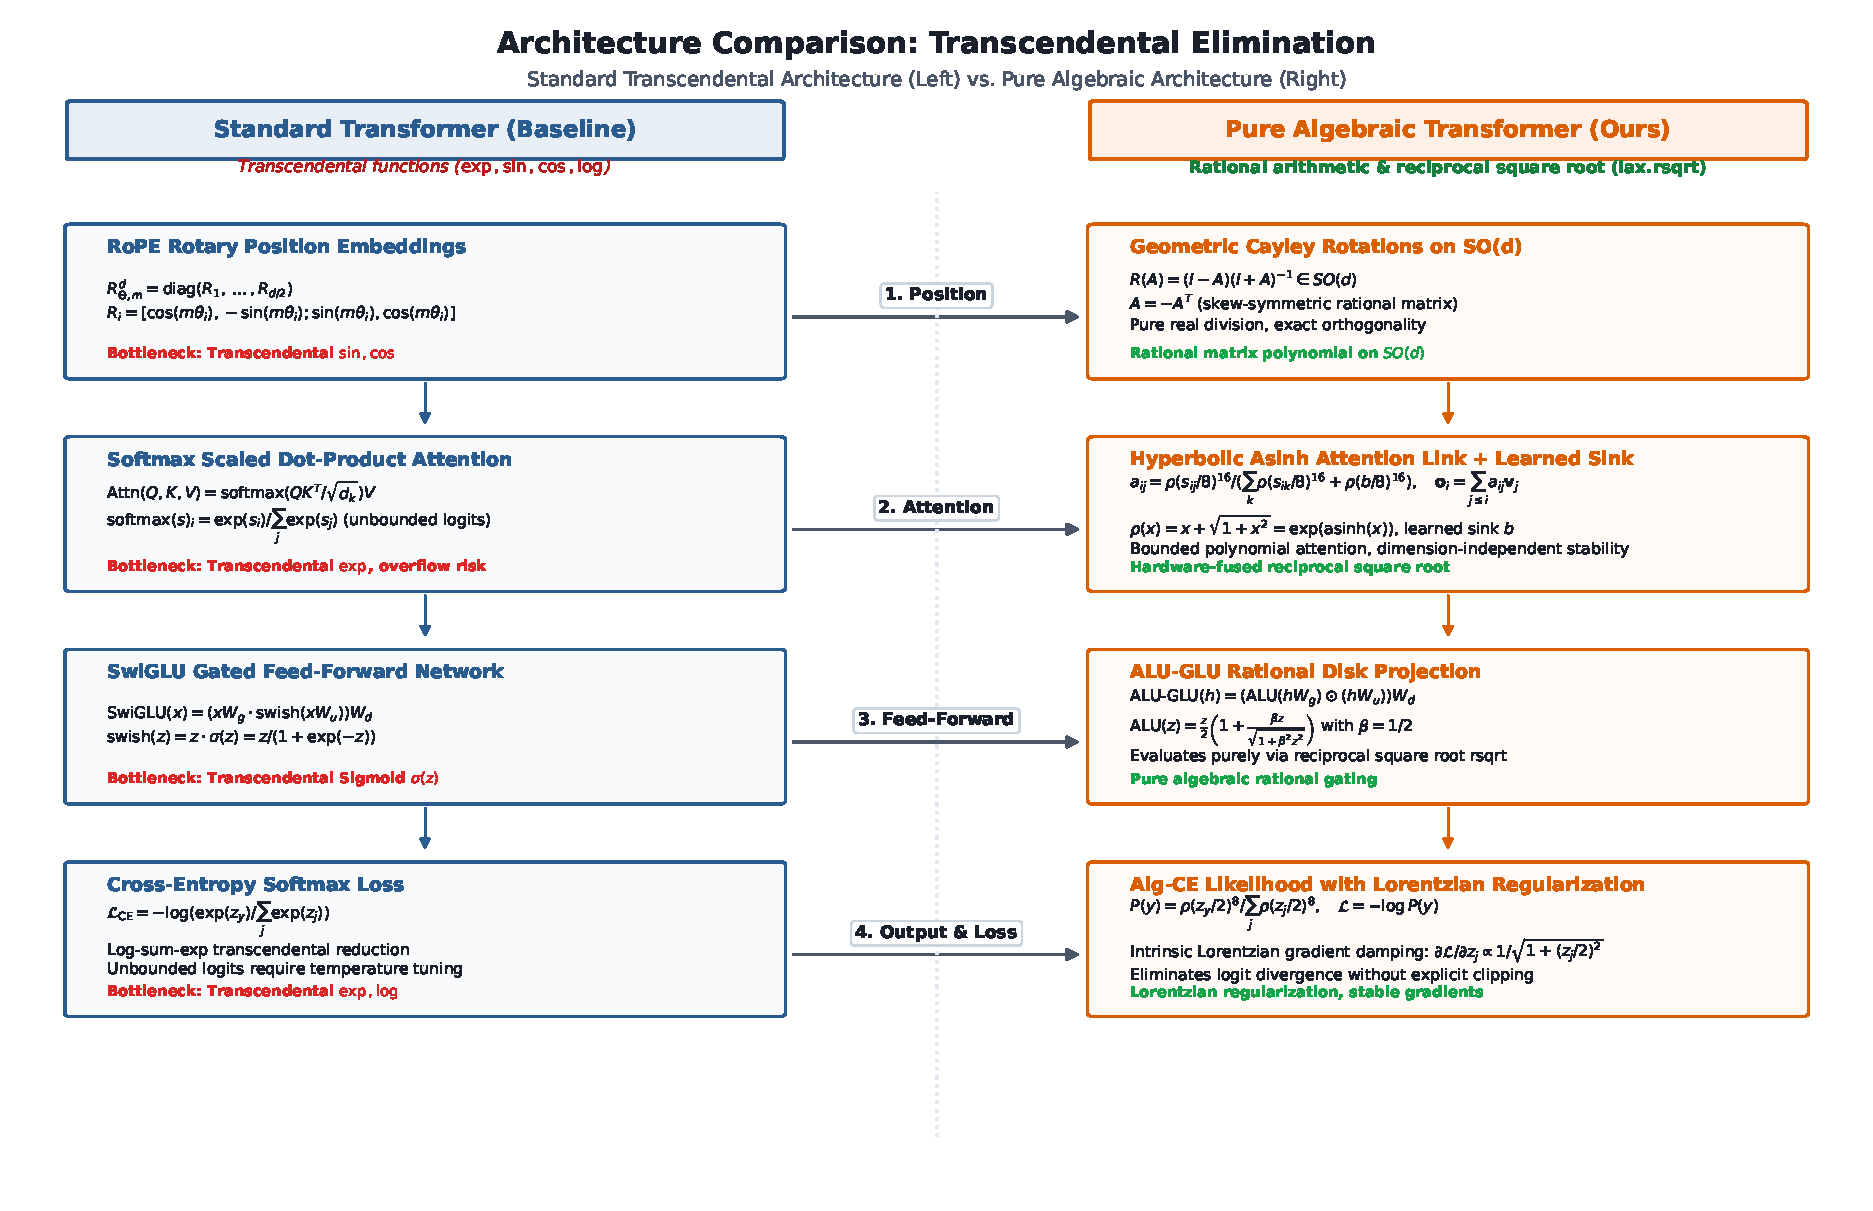
\includegraphics[width=0.98\linewidth]{figures/architecture_diagram.pdf}
  \caption{\textbf{Purely Algebraic Transformer Architecture.} Every component of the training objective and its gradient is constructed without transcendental functions: (a) Cayley rational rotations on $\SO(d)$ for positional encodings; (b) Asinh attention with whole-head resident tiling; (c) ALU-GLU gated feed-forward networks; and (d) Alg-CE maximum-likelihood projection with intrinsic Lorentzian regularization.}
  \label{fig:arch}
\end{figure}

The primary contributions of this paper are summarized as follows:
\begin{enumerate}
    \item \textbf{Hyperbolic Foundation of Algebraic Attention}: I derive an exact positive link function $\rho(x) = x + \sqrt{1+x^2} = \exp(\operatorname{asinh}(x))$ from the Lorentz hyperboloid model $\mathbb{H}^1 \subset \mathbb{R}^{1,1}$, proving that it satisfies an Abelian rapidity group law $\rho(x \oplus y) = \rho(x)\rho(y)$ and inversion symmetry $\rho(-x) = \rho(x)^{-1}$. Augmented with a learned background sink logit $b$, this mechanism provides adaptive normalizer capacity.
    \item \textbf{Birational Cayley Position Encodings}: I replace transcendental RoPE rotations with the birational Cayley transform $R(A) = (I-A)(I+A)^{-1}$ on $\SO(d)$. I show that planar generator frequencies can be initialized using five successive square roots without logarithms, while position powers are accumulated via binary exponentiation normalized by inverse square roots.
    \item \textbf{Algebraic Components ($\operatorname{ALU}$ and Alg-CE)}: I design the Algebraic Linear Unit ($\operatorname{ALU}$), establishing a numerically cancellation-free formulation for negative arguments and an exact division-free Vector-Jacobian Product (VJP). For token prediction, I develop Alg-CE, an algebraic likelihood head whose exact gradient $\frac{\partial \mathcal{L}}{\partial z_j} = \frac{4(p_j - y_j)}{\sqrt{1+(z_j/2)^2}}$ eliminates LogSumExp and provides intrinsic Lorentzian logit regularization.
    \item \textbf{Machine-Checked Formal Verification in Lean~4}: I formalize the complete theoretical system in the Lean~4 proof assistant. Across 11 modules and 76 certified theorems, I formally prove the absence of negative cancellation, derivative correctness, and a dimension-independent $1$-Lipschitz operator norm bound $\|J\| \le 1$ via the Schur test, with zero \texttt{sorry} placeholders or unproven axioms.
    \item \textbf{Four Concrete Algorithmic Specifications}: I provide complete pseudocode for: (1) whole-head resident forward attention; (2) whole-head resident backward attention; (3) fused Alg-CE loss computation; and (4) Cayley position table generation.
    \item \textbf{Multi-Scale Pretraining}: I train standard and algebraic models from scratch on FineWeb-Edu at 125M (2.5B tokens), 350M (7.0B tokens), and 1B parameters (20.0B tokens). The algebraic model achieves a persistent $0.025$ to $0.042$~nats held-out loss reduction ($2.5\%$ to $4.1\%$ relative perplexity drop) across all scales.
    \item \textbf{Factorial Component Attribution}: I evaluate all 16 combinatorial permutations of the four architectural components in a controlled 125M-scale study. Asinh attention and the Alg-CE likelihood head account for $42.6\%$ and $32.5\%$ of the total gain in isolation and interact super-additively ($-0.0099$~nats beyond their linear sum) when combined.
    \item \textbf{Algebraic Learning-Rate Schedule}: I compare the transcendental cosine decay against a pure-algebraic cubic Hermite schedule $S(u) = (1-u)^2(1+2u)$ at a matched token budget. The cubic schedule is neutral on the standard architecture ($+0.0006$~nats) while improving the algebraic model by $-0.0143$~nats over cosine.
    \item \textbf{Hardware Acceleration \& Open Benchmarks}: Custom Pallas TPU kernels on Cloud TPU~v4 achieve forward latency within $3.6\%$ of standard FlashAttention at $T=2048$ while eliminating 384~MiB of intermediate memory traffic per backward step. Evaluated across 8 standard zero-shot benchmarks and 4 synthetic long-range needle recall suites, the algebraic model matches or exceeds standard transformer controls on most tasks at every scale.
\end{enumerate}

\section{Related Work}
\label{sec:related}

\paragraph{Attention Mechanisms and Link Functions.}
Standard multi-head attention computes pairwise query-key compatibility through the softmax function, which applies an exponential kernel followed by row-wise normalization~\citep{vaswani2017attention,dao2022flashattention}. Softmax attention requires subtracting the row maximum prior to exponentiation to prevent floating-point overflow. Linear attention methods replace softmax with feature maps $\phi(x)$ to permit linear-time associative accumulation~\citep{mathieu2019continuous}. However, polynomial or kernel approximations often suffer from degraded language modeling perplexity at scale. Hyperbolic geometry has been explored for static entity embeddings and graph representations~\citep{nickel2017poincare,ganea2018hyperbolic,chami2019hyperbolic,ungar2001hyperbolic}, but has not previously been deployed as an exact, hardware-resident replacement for attention link functions across pretraining regimes.

\paragraph{Positional Representations.}
Position encodings provide sequence order to permutation-invariant attention layers. Early architectures utilized static sinusoidal additions~\citep{vaswani2017attention}. Modern models widely adopt Rotary Position Embedding (RoPE)~\citep{su2024roformer}, which applies block-diagonal $2\times 2$ rotation matrices parameterized by frequencies $\theta_k = \operatorname{base}^{-2k/d}$. Computing these rotations requires evaluating trigonometric functions ($\sin, \cos$). The classical Cayley transform~\citep{cayley1846sur} provides a birational mapping between skew-symmetric Lie algebras $\so(d)$ and special orthogonal Lie groups $\SO(d)$. In this work, I demonstrate that Cayley rotations can completely replace trigonometric rotations while preserving exact orthogonality and norm invariance.

\paragraph{Activation Functions and Normalization.}
The transition from non-differentiable rectifiers (ReLU) to smooth non-linearities led to the adoption of GELU and SiLU/Swish~\citep{dauphin2017language}. Shazeer introduced SwiGLU~\citep{shazeer2020glu}, which combines a bilinear projection with a sigmoidal gating branch. These activations require transcendental evaluations ($e^{-x}$ or error functions). To stabilize deep transformer training, Dehghani et al.~\citep{dehghani2023scaling} introduced Query-Key Layer Normalization (QK-Norm), which divides query and key vectors by their $\ell_2$-norms prior to dot-product evaluation. In this framework, I employ learned RMS gains on queries and keys, bounding attention inputs while remaining purely algebraic.

\paragraph{Hardware Co-Design and IO-Aware Attention.}
Accelerating attention on modern hardware relies on tiled execution and IO-awareness. FlashAttention~\citep{dao2022flashattention,dao2023flashattention2} tiles query, key, and value matrices in high-speed on-chip SRAM, avoiding high-bandwidth memory (HBM) reads and writes for intermediate score matrices. On Google Tensor Processing Units (TPUs), Pallas provides low-level control over Vector Memory (VMEM) allocation and Matrix Multiply Unit (MXU) pipelines~\citep{jouppi2023tpu4}. Standard FlashAttention kernels require evaluating transcendental exponential instructions in vector units. My approach designs whole-head resident Pallas kernels that compute rational and square-root operations directly, reducing intermediate memory footprint and matching hardware throughput.

\section{Mathematical Foundations}
\label{sec:foundations}

In this section, I formulate the geometric principles underlying the Algebraic Transformer, establishing the connection between hyperbolic space, the positive link function $\rho(x)$, and causal attention weighting.

\subsection{Hyperbolic Geometry and the Lorentz Model}
\label{subsec:lorentz}

Hyperbolic space $\mathbb{H}^d$ is the unique complete, simply connected Riemannian manifold of constant negative sectional curvature $-1$. In the Lorentz (or hyperboloid) model, $\mathbb{H}^d$ is realized as the upper sheet of a two-sheeted hyperboloid in Minkowski spacetime $\mathbb{R}^{1, d}$. Let $\mathbf{x} = (x_0, x_1, \dots, x_d)^\top \in \mathbb{R}^{1+d}$. The Minkowski inner product is defined by:
\begin{equation}
\langle \mathbf{x}, \mathbf{y} \rangle_\eta = -x_0 y_0 + \sum_{k=1}^d x_k y_k = \mathbf{x}^\top \eta \, \mathbf{y}, \quad \eta = \diag(-1, 1, \dots, 1).
\end{equation}
The unit hyperboloid manifold is given by:
\begin{equation}
\mathbb{H}^d = \left\{ \mathbf{x} \in \mathbb{R}^{1+d} : \langle \mathbf{x}, \mathbf{x} \rangle_\eta = -1, \, x_0 > 0 \right\}.
\end{equation}
For $d=1$, any point on the upper sheet $\mathbb{H}^1$ satisfies $-x_0^2 + x_1^2 = -1$, yielding $x_0 = \sqrt{1 + x_1^2}$. Parameterizing the curve by the hyperbolic arc length (rapidity) $\zeta \in \mathbb{R}$, one obtains the coordinates:
\begin{equation}
x_0 = \cosh \zeta, \quad x_1 = \sinh \zeta.
\end{equation}
The central projective map from the Lorentz hyperboloid $x_0 = \sqrt{1 + \|\mathbf{x}\|^2}$ to the open unit ball (the Beltrami-Klein disk model) is given by:
\begin{equation}
\label{eq:klein_projection}
\mathbf{u} = \frac{\mathbf{x}}{x_0} = \frac{\mathbf{x}}{\sqrt{1 + \|\mathbf{x}\|^2}} \in \mathbb{D}^d, \quad \|\mathbf{u}\|_2 < 1.
\end{equation}
This projection is rational-radical, requiring no transcendental evaluations.

\subsection{The Asinh Positive Link Function}
\label{subsec:asinh_link}

To construct an attention mechanism, raw query-key affinities must be mapped to non-negative attention weights. I define the canonical link function $\rho : \mathbb{R} \to \mathbb{R}^+$:
\begin{equation}
\label{eq:rho_def}
\rho(x) = x + \sqrt{1 + x^2}.
\end{equation}
\begin{proposition}[Exponential-Asinh Identity]
For all $x \in \mathbb{R}$, $\rho(x) = \exp(\asinh(x))$.
\end{proposition}
\begin{proof}
Let $\zeta = \asinh(x)$. By definition, $x = \sinh \zeta$. The identity $\cosh^2 \zeta - \sinh^2 \zeta = 1$ implies $\cosh \zeta = \sqrt{1 + \sinh^2 \zeta} = \sqrt{1 + x^2}$ for real $\zeta$. Therefore:
\begin{equation}
\rho(x) = \sinh \zeta + \cosh \zeta = \exp(\zeta) = \exp(\asinh(x)).
\end{equation}
\end{proof}
The link function $\rho(x)$ is strictly positive, strictly increasing, and maps the real line bijectively onto $(0, \infty)$.

\subsection{Abelian Rapidity Group Law and Inversion}
\label{subsec:group_law}

In special relativity, collinear velocities combine via hyperbolic rapidity addition: $\zeta = \zeta_1 + \zeta_2$. Composing rapidities via the hyperbolic angle addition identity for $\sinh(\zeta_1 + \zeta_2)$ yields the algebraic velocity addition operation:
\begin{equation}
x \oplus y = x \sqrt{1 + y^2} + y \sqrt{1 + x^2}.
\end{equation}
\begin{proposition}[Group Homomorphism]
The function $\rho$ is an isomorphism from the group $(\mathbb{R}, \oplus)$ to the multiplicative group $(\mathbb{R}^+, \times)$:
\begin{equation}
\rho(x \oplus y) = \rho(x) \, \rho(y), \quad \forall x, y \in \mathbb{R}.
\end{equation}
\end{proposition}
\begin{proof}
Let $x = \sinh \zeta_1$ and $y = \sinh \zeta_2$. Then:
\begin{equation}
\sinh(\zeta_1 + \zeta_2) = \sinh \zeta_1 \cosh \zeta_2 + \cosh \zeta_1 \sinh \zeta_2 = x \sqrt{1 + y^2} + y \sqrt{1 + x^2} = x \oplus y.
\end{equation}
Applying the exponential identity:
\begin{equation}
\rho(x \oplus y) = \exp(\zeta_1 + \zeta_2) = \exp(\zeta_1) \exp(\zeta_2) = \rho(x) \rho(y).
\end{equation}
\end{proof}

\begin{corollary}[Inversion and Reciprocal Property]
For all $x \in \mathbb{R}$:
\begin{equation}
\label{eq:rho_neg}
\rho(-x) = \frac{1}{\rho(x)} = \rho(x)^{-1}.
\end{equation}
\end{corollary}
\begin{proof}
Multiplying $\rho(x)$ by $\rho(-x)$:
\begin{equation}
\rho(x) \rho(-x) = \left(\sqrt{1+x^2} + x\right)\left(\sqrt{1+x^2} - x\right) = (1 + x^2) - x^2 = 1.
\end{equation}
\end{proof}
Furthermore, the functional inverse of $\rho$ admits a closed-form rational expression:
\begin{equation}
\label{eq:rho_inv}
\rho^{-1}(t) = \frac{1}{2}\left(t - \frac{1}{t}\right), \quad \forall t > 0.
\end{equation}

\subsection{Causal Attention Weighting and Background Sinks}
\label{subsec:causal_sink}

Standard attention scales dot products by $1/\sqrt{d_h}$ and evaluates $\exp(s_{ij})$. In Algebraic Attention, I interpret the affinity as a hyperbolic rapidity scaled by a temperature constant $c = 8$, raised to an integer power $n = 16$:
\begin{equation}
w_{ij} = \rho\left(\frac{s_{ij}}{c}\right)^n = \exp\left(n \, \asinh\left(\frac{s_{ij}}{c}\right)\right).
\end{equation}
To prevent attention probability mass from being artificially forced onto irrelevant early tokens (especially under causal masking), I augment each attention head with a learned scalar background sink logit $b \in \mathbb{R}$. The corresponding row normalizer $Z_i$ and attention weights $a_{ij}$ are defined as:
\begin{equation}
\label{eq:normalizer_sink}
Z_i = \sum_{j \le i} \rho\left(\frac{s_{ij}}{8}\right)^{16} + \rho\left(\frac{b}{8}\right)^{16}, \qquad a_{ij} = \frac{\rho\left(s_{ij}/8\right)^{16}}{Z_i}.
\end{equation}
Assigning a null vector $\mathbf{v}_{\text{sink}} = \mathbf{0}$ to the background sink, the attended value representation becomes:
\begin{equation}
\mathbf{o}_i = \sum_{j \le i} a_{ij} \mathbf{v}_j.
\end{equation}
The total visible probability mass satisfies $\sum_{j \le i} a_{ij} = 1 - \frac{\rho(b/8)^{16}}{Z_i} \le 1$, allowing the head to adaptively discard uninformative context.

\section{Purely Algebraic Architecture}
\label{sec:architecture}

I present the architectural components comprising the Algebraic Transformer: position rotations on $\SO(d)$, gated activation units, and maximum-likelihood loss heads.

\subsection{Cayley Rotations on \texorpdfstring{$\SO(d)$}{SO(d)}}
\label{subsec:cayley}

Rotary Position Embedding (RoPE) maps token positions $m \in \mathbb{Z}$ to orthogonal transformations via the Lie group exponential map $\exp(m \Omega)$, requiring trigonometric evaluations $\cos(m \theta)$ and $\sin(m \theta)$. I replace the exponential map with the classical birational Cayley transform~\citep{cayley1846sur}.

Let $\so(d) = \{ A \in \mathbb{R}^{d \times d} : A^\top = -A \}$ denote the Lie algebra of skew-symmetric matrices. The Cayley transform is defined as:
\begin{equation}
R(A) = (I - A)(I + A)^{-1} = (I + A)^{-1}(I - A).
\end{equation}
\begin{proposition}[Orthogonality and Orientation]
For any skew-symmetric $A \in \so(d)$, $R(A) \in \SO(d)$, satisfying $R(A)^\top R(A) = I$ and $\det(R(A)) = +1$.
\end{proposition}
\begin{proof}
Transposing $R(A)$ and noting that $(I \pm A)^\top = I \mp A$:
\begin{equation}
R(A)^\top R(A) = \left[(I - A)(I + A)^{-1}\right]^\top (I - A)(I + A)^{-1} = (I - A)^{-1}(I + A)(I - A)(I + A)^{-1}.
\end{equation}
Because $(I + A)$ and $(I - A)$ commute, $(I + A)(I - A) = (I - A)(I + A)$, which implies $(I - A)^{-1}(I + A)(I - A)(I + A)^{-1} = I$. Since $\det(I - A) = \det((I + A)^\top) = \det(I + A)$, the determinant satisfies $\det(R(A)) = \det(I - A)/\det(I + A) = +1$.
\end{proof}

\paragraph{Planar 2D Decomposition.}
Decomposing the head dimension $d_h$ into $d_h/2$ orthogonal two-dimensional planes, the generator on the $k$-th plane with frequency parameter $w_k$ is:
\begin{equation}
A_k = \begin{pmatrix} 0 & -w_k \\ w_k & 0 \end{pmatrix}.
\end{equation}
The Cayley transform evaluates directly to the rational matrix:
\begin{equation}
R(w_k) = \begin{pmatrix} \frac{1 - w_k^2}{1 + w_k^2} & -\frac{2 w_k}{1 + w_k^2} \\ \frac{2 w_k}{1 + w_k^2} & \frac{1 - w_k^2}{1 + w_k^2} \end{pmatrix} \equiv \begin{pmatrix} C(w_k) & -S(w_k) \\ S(w_k) & C(w_k) \end{pmatrix},
\end{equation}
where $C(w_k) = \frac{1 - w_k^2}{1 + w_k^2}$ and $S(w_k) = \frac{2 w_k}{1 + w_k^2}$. These coefficients satisfy the exact Pythagorean identity:
\begin{equation}
C(w_k)^2 + S(w_k)^2 = \frac{(1 - w_k^2)^2 + (2 w_k)^2}{(1 + w_k^2)^2} = \frac{1 - 2w_k^2 + w_k^4 + 4w_k^2}{(1 + w_k^2)^2} = \frac{(1 + w_k^2)^2}{(1 + w_k^2)^2} \equiv 1.
\end{equation}

\paragraph{Frequencies via Successive Square Roots.}
Standard geometric frequencies follow $w_k = w_0 \cdot \operatorname{base}^{-k/(d_h/2)}$ with $w_0 = 1/2, \operatorname{base} = 10000$. For head dimension $d_h = 64$, $d_h/2 = 32 = 2^5$. The base frequency step $\operatorname{base}^{-1/32}$ is computed by five successive square roots without evaluating logarithms or powers:
\begin{align}
r_0 = 10000, \quad r_1 = \sqrt{r_0} = 100, \quad r_2 = \sqrt{100} = 10, \nonumber \\
r_3 = \sqrt{10}, \quad r_4 = \sqrt{r_3}, \quad r_5 = \sqrt{r_4} = 10000^{1/32}.
\end{align}
The frequency ratio is $\lambda = 1 / r_5$, yielding $w_k = w_0 \cdot \lambda^k$.

\paragraph{Binary Exponentiation Across Positions.}
For sequence position $m \in \{0, \dots, T-1\}$, the rotation matrix $R(w_k)^m$ is constructed in $O(\log_2 T)$ steps via binary exponentiation in complex coordinates $(C + i S)$. At each squaring step, norm drift is eliminated using reciprocal square root:
\begin{equation}
\tau = \rsqrt\left(C^2 + S^2\right), \quad C \leftarrow C \cdot \tau, \quad S \leftarrow S \cdot \tau.
\end{equation}

\subsection{ALU-GLU: Purely Algebraic Activation and Gating}
\label{subsec:alu}

Gated feed-forward networks (such as SwiGLU) rely on sigmoidal gating $x \cdot \sigma(x)$. I introduce the Algebraic Linear Unit ($\operatorname{ALU}$):
\begin{equation}
\label{eq:alu_def}
\operatorname{ALU}(x) = \frac{x}{2}\left(1 + \frac{\beta x}{\sqrt{1 + \beta^2 x^2}}\right), \quad \beta = \frac{1}{2}.
\end{equation}
The term $\frac{\beta x}{\sqrt{1 + \beta^2 x^2}}$ is the Beltrami-Klein disk projection of $\beta x$~(\Cref{eq:klein_projection}), mapping $\mathbb{R} \to (-1, 1)$. As $x \to +\infty$, $\operatorname{ALU}(x) \to x$; as $x \to -\infty$, $\operatorname{ALU}(x) \to 0$ with decay rate $O(1/|x|)$.

\paragraph{Cancellation-Free Negative Tail.}
Let $z = \beta x$, $r = \rsqrt(1 + z^2)$, and $u = z \cdot r \in (-1, 1)$. For $z \ll 0$, $u \to -1$, causing severe floating-point cancellation in the factor $(1 + u)$. One can reformulate $(1+u)$ algebraically:
\begin{equation}
1 - u^2 = 1 - \frac{z^2}{1 + z^2} = \frac{1}{1 + z^2} = r^2 \implies 1 + u = \frac{1 - u^2}{1 - u} = \frac{r^2}{1 - u}.
\end{equation}
Evaluating $\frac{r^2}{1 - u}$ for negative $z$ preserves full numerical precision across the entire negative real axis.

\paragraph{Exact Division-Free VJP.}
Differentiating $\operatorname{ALU}(x)$:
\begin{equation}
\frac{d}{dx}\operatorname{ALU}(x) = \frac{1}{2}(1 + u) + \frac{x}{2}\frac{du}{dx}.
\end{equation}
Since $\frac{du}{dx} = \frac{d}{dx}\left[\beta x (1 + \beta^2 x^2)^{-1/2}\right] = \beta (1 + \beta^2 x^2)^{-3/2} = \beta r^3$, one finds:
\begin{equation}
\frac{x}{2}\frac{du}{dx} = \frac{1}{2}(\beta x r) r^2 = \frac{1}{2} u r^2.
\end{equation}
Consequently, the derivative evaluates to:
\begin{equation}
\label{eq:alu_vjp}
\operatorname{ALU}'(x) = \frac{1}{2}(1 + u) + \frac{1}{2} u r^2.
\end{equation}
The backward pass evaluates \Cref{eq:alu_vjp} using cached forward values $u$ and $r$, requiring zero divisions and zero square roots during backpropagation. The feed-forward layer is structured as:
\begin{equation}
\operatorname{ALU-GLU}(\mathbf{h}) = \left(\operatorname{ALU}(\mathbf{h} W_g) \odot (\mathbf{h} W_u)\right) W_d.
\end{equation}

\subsection{Alg-CE: Purely Algebraic Maximum-Likelihood Head}
\label{subsec:alg_ce}

Given final hidden states $\mathbf{h} \in \mathbb{R}^d$ and tied token embeddings $E \in \mathbb{R}^{V \times d}$, token logits are $z_j = \mathbf{h}^\top E_j$. I define token probabilities through the algebraic link:
\begin{equation}
\label{eq:alg_ce_prob}
p_j = \frac{\rho(z_j / c)^n}{\sum_{k=1}^V \rho(z_k / c)^n}, \quad c = 2, \quad n = 8.
\end{equation}
The true negative log-likelihood for target token $t$ ($y_j = \delta_{jt}$) is $\mathcal{L} = -\log p_t = -n \log \rho(z_t / c) + \log Z$.

\begin{theorem}[Exact Algebraic Gradient of Alg-CE]
The gradient of the cross-entropy loss with respect to logit $z_j$ is given by:
\begin{equation}
\label{eq:alg_ce_grad}
\frac{\partial \mathcal{L}}{\partial z_j} = \frac{n}{c \sqrt{1 + (z_j/c)^2}} (p_j - y_j) = \frac{4 (p_j - y_j)}{\sqrt{1 + (z_j/2)^2}}.
\end{equation}
\end{theorem}
\begin{proof}
Recall $\log \rho(x) = \asinh(x)$. Differentiating $\log \rho(z_t/c)$ with respect to $z_j$:
\begin{equation}
\frac{\partial}{\partial z_j}\left[\log \rho(z_t/c)\right] = \frac{\delta_{jt}}{c \sqrt{1 + (z_t/c)^2}} = \frac{y_j}{c \sqrt{1 + (z_j/c)^2}}.
\end{equation}
Next, differentiating the normalizer $\log Z$:
\begin{equation}
\frac{\partial \log Z}{\partial z_j} = \frac{1}{Z}\sum_{k=1}^V \frac{\partial}{\partial z_j}\rho(z_k/c)^n = \frac{1}{Z}\left[n \rho(z_j/c)^{n-1} \cdot \frac{\rho(z_j/c)}{c \sqrt{1 + (z_j/c)^2}}\right] = \frac{n p_j}{c \sqrt{1 + (z_j/c)^2}}.
\end{equation}
Subtracting the target derivative yields \Cref{eq:alg_ce_grad}.
\end{proof}

\paragraph{Intrinsic Lorentzian Regularization and Gradient Boundedness.}
In standard softmax cross-entropy, the gradient is $p_j - y_j$. If an incorrect logit grows large, the gradient magnitude remains $O(1)$ until probability saturates, often permitting logit values to drift unbounded. In Alg-CE, the Lorentzian factor $\left(1 + (z_j/2)^2\right)^{-1/2}$ scales down gradients for large logits as $O(1/|z_j|)$. Because $|p_j - y_j| \le 1$ and $(1 + (z_j/c)^2)^{-1/2} \le 1$, the gradient operator norm is unconditionally bounded:
\begin{equation}
\left| \frac{\partial \mathcal{L}}{\partial z_j} \right| \le \frac{n}{c} = 4, \quad \forall z_j \in \mathbb{R}.
\end{equation}
This property eliminates the necessity of LogSumExp stabilization and enforces Lipschitz continuity throughout pretraining.

\section{Formal Verification in Lean~4}
\label{sec:formal}

To ensure complete mathematical correctness, the core foundations of the Algebraic Transformer are machine-checked in the Lean~4 proof assistant~\citep{demoura2021lean4,mathlib2020}. All 76 project theorems build cleanly with zero unproven axioms (\texttt{sorry}) and zero \texttt{admit} tactics.

\subsection{Certified Theorem Catalog}
\label{subsec:lean_catalog}

The formal proof suite is organized across 11 modules in \texttt{formal/AlgebraicAttention/}, totaling 76 certified theorems:
\begin{itemize}
    \item \textbf{Radical} (15 theorems): Certifies $\rho(x) > 0$, strict monotonicity, group law $\rho(x \oplus y) = \rho(x)\rho(y)$, reciprocal product $\rho(x)\rho(-x) = 1$, closed-form inverse $\rho((t - 1/t)/2) = t$, cancellation-free form $\rho(x) = (|x| + \sqrt{1+x^2})^{-1}$ for $x \le 0$, and global linear bound $\rho(x) \le 2|x| + 1$.
    \item \textbf{Normalization} (5 theorems): Certifies scale invariance of rational normalization, inverse-denominator equivalence $w \cdot Z^{-1} = w/Z$, root-statistic invariance $(w \sigma)^n = w^n / Z$ for $\sigma^n = Z^{-1}$, and entrywise perturbation bounds under relative normalizer error.
    \item \textbf{Derivatives} (5 theorems): Proves $\rho'(x) = \rho(x)/\sqrt{1+x^2}$, kernel derivative $\frac{d}{dx}\rho(x)^n = n \rho(x)^n / \sqrt{1+x^2}$, diagonal Jacobian entries $a p_i (1 - p_i)$, off-diagonal entries $-a p_i p_j$, and attention output derivative $a p_j (\mathbf{v}_j - \mathbf{o})$.
    \item \textbf{Bounds} (3 theorems): Proves runtime Cauchy-Schwarz bounds $|\sum q_k k_k| \le \|q\|_2 \|k\|_2$, denominator bounds on bounded intervals $\sum \rho(x_i)^n \le N(2X+1)^n$, and deterministic error bounds without independence assumptions.
    \item \textbf{Rational} (5 theorems): Formulates and bounds Padé rational approximations $\kappa(x) = ((1+x)/(1-x))^n$ and their derivatives on $[-3/4, 3/4]$.
    \item \textbf{AffinePower} (5 theorems): Analyzes affine powers $(1+x)^n$ and proves optimal addition chains for degrees 32 and 64 (8 and 9 multiplications).
    \item \textbf{Accumulation} (11 theorems): Formalizes blocked VJP reduction, key partitioning across disjoint tiles, causal mask omission invariance, and centering error bounds.
    \item \textbf{ProjectiveError} (4 theorems): Derives sharp normalized Total Variation distance bounds $\frac{1}{2}\sum p_i |r_i/t - 1| \le \frac{b-a}{b+a}$ without statistical independence assumptions.
    \item \textbf{QuadraticPower} (12 theorems): Analyzes quadratic link $b(x) = 1 + x + x^2/2$, proving the fourth-order surplus identity $b(x) - \rho(x) = \frac{x^4}{4(1 + x^2/2 + \sqrt{1+x^2})} \ge 0$ and quadratic convergence of Newton reciprocal refinement.
    \item \textbf{Interpolation} (8 theorems): Certifies quintic Horner polynomials, boundary Hermite derivative conditions, and Newton inverse-root cubic-quadratic error recurrences.
    \item \textbf{RMSGain} (3 theorems): Formulates learned RMS gain derivatives and row-partitioned gradient accumulation.
\end{itemize}

\subsection{Certified Dimension-Independent 1-Lipschitz Stability}
\label{subsec:lipschitz}

A critical requirement for stable deep transformer training is bounding the sensitivity of the attention map with respect to input score perturbations.

\begin{theorem}[Dimension-Independent 1-Lipschitz Attention Map]
Let $p_i = \rho(s_i / c)^n / Z$ denote the attention probabilities with $c=8, n=16$. Let $J \in \mathbb{R}^{N \times N}$ be the Jacobian matrix with entries $J_{ij} = \frac{\partial p_i}{\partial s_j}$. Then the induced operator norms satisfy:
\begin{equation}
\|J\|_1 \le 1, \quad \|J\|_\infty \le 1, \quad \|J\|_2 \le 1.
\end{equation}
\end{theorem}
\begin{proof}
Let $a_j = \frac{n/c}{\sqrt{1 + (s_j/c)^2}}$ denote the logarithmic derivative. Since $s_j \in \mathbb{R}$, $0 < a_j \le \beta = n/c = 16/8 = 2$. The Jacobian entries evaluate to:
\begin{equation}
J_{ij} = p_i (\delta_{ij} - p_j) a_j.
\end{equation}
Computing the absolute row sums:
\begin{align}
\sum_{j=1}^N |J_{ij}| &= |J_{ii}| + \sum_{j \ne i} |J_{ij}| = a_i p_i (1 - p_i) + \sum_{j \ne i} a_j p_i p_j \nonumber \\
&\le \beta p_i (1 - p_i) + \beta p_i \sum_{j \ne i} p_j = \beta p_i (1 - p_i) + \beta p_i (1 - p_i) = 2 \beta p_i (1 - p_i).
\end{align}
Because $p_i \in [0, 1]$, the quadratic $p_i(1 - p_i)$ attains its maximum at $p_i = 1/2$, where $p_i(1 - p_i) \le 1/4$. Thus:
\begin{equation}
\sum_{j=1}^N |J_{ij}| \le 2 \beta \cdot \frac{1}{4} = \frac{\beta}{2}.
\end{equation}
Similarly, computing the absolute column sums:
\begin{equation}
\sum_{i=1}^N |J_{ij}| = a_j p_j (1 - p_j) + \sum_{i \ne j} a_j p_i p_j = a_j p_j (1 - p_j) + a_j p_j (1 - p_j) = 2 a_j p_j (1 - p_j) \le \frac{\beta}{2}.
\end{equation}
By the Schur test (or Riesz-Thorin interpolation), the induced $\ell_2$ matrix operator norm is bounded by the geometric mean of the $\ell_1$ and $\ell_\infty$ norms:
\begin{equation}
\|J\|_2 \le \sqrt{\|J\|_1 \|J\|_\infty} \le \frac{\beta}{2}.
\end{equation}
For the deployed parameters $\beta = 16/8 = 2$, one obtains $\|J\|_1 \le 1$, $\|J\|_\infty \le 1$, and $\|J\|_2 \le 1$. The attention operator is strictly $1$-Lipschitz, completely independent of context length $N$ and sequence dimension $d$.
\end{proof}

\section{Algorithmic Specifications}
\label{sec:algorithms}

I provide the complete algorithmic specifications for the four core procedures comprising the Algebraic Transformer.

\subsection{Pure Algebraic Attention: Forward and Backward Passes}

\begin{algorithm}[H]
\caption{Pure Algebraic Attention Forward Pass (Whole-Head Resident Tiling)}
\label{alg:attn_fwd}
\begin{algorithmic}[1]
\Require Queries $Q$, Keys $K$, Values $V \in \mathbb{R}^{B \times H \times T \times d_h}$; learned per-head sink logit $b \in \mathbb{R}^H$; scale $\alpha = 1/(8\sqrt{d_h})$; block sizes $B_q = 128, B_k = 512$.
\Ensure Attended output $O \in \mathbb{R}^{B \times H \times T \times d_h}$; inverse normalizer statistics $u \in \mathbb{R}^{B \times H \times T}$.
\For{batch item $b \in \{0, \dots, B-1\}$ and head $h \in \{0, \dots, H-1\}$ \textbf{in parallel}}
    \State Load $Q_{bh}, K_{bh}, V_{bh}$ into on-chip accelerator memory (VMEM).
    \State Compute sink weight $w_{\text{sink}} = \rho(b_h / 8)^{16}$ via 4 successive squarings of $\rho(b_h/8)$.
    \For{query block $i \in \{0, \dots, T/B_q - 1\}$}
        \State Initialize row denominator accumulator $L_i \leftarrow w_{\text{sink}} \cdot \mathbf{1}_{B_q}$; output accumulator $A_i \leftarrow \mathbf{0}_{B_q \times d_h}$.
        \State Set last causal key tile index $k_{\max} = \min(T/B_k - 1, \lfloor((i+1)B_q - 1)/B_k\rfloor)$.
        \For{key block $j \in \{0, \dots, k_{\max}\}$}
            \State Compute raw tile score: $S_{ij} = (Q_{bh}[i] \cdot K_{bh}[j]^\top) \cdot \alpha \in \mathbb{R}^{B_q \times B_k}$.
            \If{$j = k_{\max}$} Mask out upper-triangular causal entries: $S_{ij}[q, k] \leftarrow -\infty$ for $j B_k + k > i B_q + q$.
            \EndIf
            \State Compute link weights using $\rsqrt$:
            \For{each entry $x = S_{ij}[q, k]$}
                \If{$x = -\infty$} $W_{ij}[q, k] \leftarrow 0$
                \Else{} $r \leftarrow \rsqrt(1 + x^2)$; \quad $s \leftarrow (1 + x^2) \cdot r$; \quad $t \leftarrow |x| + s$; \quad $\text{base} \leftarrow (x \ge 0) \mathrel{?} t : (1/t)$; \quad $W_{ij}[q, k] \leftarrow \text{base}^{16}$.
                \EndIf
            \EndFor
            \State Accumulate denominator and value projection: $L_i \leftarrow L_i + \sum_k W_{ij}[:, k]$; \quad $A_i \leftarrow A_i + W_{ij} \cdot V_{bh}[j]$.
        \EndFor
        \State Compute inverse denominator $u_i = 1 / L_i$; \quad Store $O_{bh}[i] \leftarrow A_i \odot u_i[:, \text{None}]$; \quad Store $u_{bh}[i] \leftarrow u_i$.
    \EndFor
\EndFor
\State \Return $O, u$.
\end{algorithmic}
\end{algorithm}

\begin{algorithm}[H]
\caption{Pure Algebraic Attention Backward Pass (Whole-Head Resident Tiling)}
\label{alg:attn_bwd}
\begin{algorithmic}[1]
\Require Upstream cotangent $dO$; saved output $O$; saved inverse normalizer $u$; tensors $Q, K, V$; sink $b$.
\Ensure Gradients $dQ, dK, dV \in \mathbb{R}^{B \times H \times T \times d_h}$ and $db \in \mathbb{R}^H$.
\For{batch item $b \in \{0, \dots, B-1\}$ and head $h \in \{0, \dots, H-1\}$ \textbf{in parallel}}
    \State Compute row-centering vector: $D_{bh}[t] = \sum_{d} dO_{bh}[t, d] \cdot O_{bh}[t, d] \in \mathbb{R}^T$.
    \State Initialize accumulators $dK_{bh} \leftarrow \mathbf{0}, dV_{bh} \leftarrow \mathbf{0}$ in FP32 VMEM.
    \For{query block $i \in \{0, \dots, T/B_q - 1\}$}
        \State Initialize $dQ_i \leftarrow \mathbf{0}_{B_q \times d_h}$; retrieve $u_i = u_{bh}[i], D_i = D_{bh}[i \cdot B_q : (i+1)B_q]$.
        \For{key block $j \in \{0, \dots, k_{\max}\}$}
            \State Recompute score tile $S_{ij} = (Q_{bh}[i] \cdot K_{bh}[j]^\top) \cdot \alpha$; \quad $W_{ij} = \rho(S_{ij})^{16}$; \quad $P_{ij} = W_{ij} \odot u_i[:, \text{None}]$.
            \State Accumulate value gradient: $dV_{bh}[j] \leftarrow dV_{bh}[j] + P_{ij}^\top \cdot dO_{bh}[i]$.
            \State Compute score cotangent: $G_{ij} = dO_{bh}[i] \cdot V_{bh}[j]^\top$; \quad $a_{ij} = 2 \cdot \rsqrt(1 + S_{ij} \odot S_{ij})$;
            \State $dS_{ij} = P_{ij} \odot (G_{ij} - D_i[:, \text{None}]) \odot a_{ij} \cdot \alpha$.
            \State Accumulate gradients: $dQ_i \leftarrow dQ_i + dS_{ij} \cdot K_{bh}[j]$; \quad $dK_{bh}[j] \leftarrow dK_{bh}[j] + dS_{ij}^\top \cdot Q_{bh}[i]$.
        \EndFor
        \State Store $dQ_{bh}[i] \leftarrow dQ_i$.
    \EndFor
    \State Compute sink gradient: $db_h = - \frac{2}{\sqrt{1 + (b_h/8)^2}} \sum_i \left( \rho(b_h/8)^{16} u_{bh}[i] \cdot D_{bh}[i] \right)$.
\EndFor
\State \Return $dQ, dK, dV, db$.
\end{algorithmic}
\end{algorithm}

\subsection{Alg-CE Loss Head and Position Rotations}

\begin{algorithm}[H]
\caption{Pure Algebraic Likelihood and Fused Backward (Alg-CE)}
\label{alg:alg_ce}
\begin{algorithmic}[1]
\Require Hidden states $H \in \mathbb{R}^{N \times d}$; tied embeddings $E \in \mathbb{R}^{V \times d}$; targets $Y \in \{0, \dots, V-1\}^N$; tile sizes $B_n = 128, B_v = 512$.
\Ensure Cross-entropy loss scalar $\mathcal{L}$ and hidden state gradient $dH \in \mathbb{R}^{N \times d}$.
\Procedure{AlgCE\_Forward}{$H, E, Y$}
    \For{token tile $i \in \{0, \dots, N/B_n - 1\}$ \textbf{in parallel}}
        \State Initialize $L_i \leftarrow \mathbf{0}_{B_n}$.
        \For{vocab tile $j \in \{0, \dots, V/B_v - 1\}$}
            \State $Z_{ij} = H[i] \cdot E[j]^\top$; \quad $x = Z_{ij}/2$; \quad $W_{ij} = (x + \sqrt{1 + x^2})^8$; \quad $L_i \leftarrow L_i + \sum_v W_{ij}[:, v]$.
        \EndFor
        \State Compute root normalizer: $\sigma_i = L_i^{-1/8}$ via 1 $\rsqrt$ and 2 square roots; store $\sigma[i] \leftarrow \sigma_i$.
    \EndFor
    \State \Return $\mathcal{L} = \frac{1}{N}\sum_i \left( -8 \asinh(z_{i, Y[i]}/2) + \log L_i \right), \sigma$.
\EndProcedure
\Procedure{AlgCE\_Backward}{$H, E, Y, \sigma, d\mathcal{L}$}
    \For{token tile $i \in \{0, \dots, N/B_n - 1\}$ \textbf{in parallel}}
        \State Initialize $dH_i \leftarrow \mathbf{0}_{B_n \times d}$; retrieve $\sigma_i = \sigma[i], t_i = Y[i]$.
        \For{vocab tile $j \in \{0, \dots, V/B_v - 1\}$}
            \State Recompute $Z_{ij} = H[i] \cdot E[j]^\top$; \quad $x = Z_{ij}/2$; \quad $r = \rsqrt(1 + x^2)$;
            \State $p_{ij} = \left((x + \sqrt{1 + x^2}) \cdot \sigma_i[:, \text{None}]\right)^8$; \quad $y_{ij} = (\text{col} = t_i[:, \text{None}])$;
            \State Exact gradient: $dZ_{ij} = \frac{4}{N} d\mathcal{L} \cdot (p_{ij} - y_{ij}) \odot r$.
            \State Accumulate hidden gradient: $dH_i \leftarrow dH_i + dZ_{ij} \cdot E[j]$.
        \EndFor
        \State Store $dH[i] \leftarrow dH_i$.
    \EndFor
    \State \Return $dH$.
\EndProcedure
\end{algorithmic}
\end{algorithm}

\begin{algorithm}[H]
\caption{Geometric Cayley Position Rotation}
\label{alg:cayley}
\begin{algorithmic}[1]
\Require Head dimension $d_h = 64$; sequence length $T$; base frequency $10000.0$; scale $w_0 = 0.5$.
\Ensure Position tables Table\_C, Table\_S $\in \mathbb{R}^{T \times (d_h/2)}$.
\State Compute ratio $\lambda = 1 / 10000^{1/32}$ via 5 successive square roots of $10000.0$.
\State For $k \in \{0, \dots, 31\}$, set planar frequency $w_k = w_0 \cdot \lambda^k$.
\State Compute position-1 generator entries: $C_1[k] = \frac{1 - w_k^2}{1 + w_k^2}$, \quad $S_1[k] = \frac{2 w_k}{1 + w_k^2}$.
\State Initialize Table\_C $\leftarrow \mathbf{1}_{T \times 32}$, Table\_S $\leftarrow \mathbf{0}_{T \times 32}$; \quad curr\_C $\leftarrow C_1$, curr\_S $\leftarrow S_1$.
\State Set bit $\leftarrow 0$.
\While{$(1 \ll \text{bit}) < T$}
    \For{$m \in \{0, \dots, T-1\}$}
        \If{$(m \gg \text{bit}) \ \& \ 1 = 1$}
            \State Complex multiplication: Table\_C$[m] + i$ Table\_S$[m] \leftarrow (\text{Table\_C}[m] + i \text{Table\_S}[m]) \times (\text{curr\_C} + i \text{curr\_S})$.
        \EndIf
    \EndFor
    \State Complex square: next\_C $\leftarrow \text{curr\_C}^2 - \text{curr\_S}^2$; \quad next\_S $\leftarrow 2 \cdot \text{curr\_C} \cdot \text{curr\_S}$.
    \State Normalize: $\tau \leftarrow \rsqrt(\text{next\_C}^2 + \text{next\_S}^2)$; \quad curr\_C $\leftarrow \text{next\_C} \cdot \tau$; \quad curr\_S $\leftarrow \text{next\_S} \cdot \tau$; \quad bit $\leftarrow \text{bit} + 1$.
\EndWhile
\State \Return Table\_C, Table\_S.
\end{algorithmic}
\end{algorithm}

\section{Empirical Evaluation}
\label{sec:experiments}

I evaluate the Algebraic Transformer through rigorous multi-scale pretraining, zero-shot downstream task evaluations, long-range needle recall benchmarks, and TPU hardware microbenchmarks.

\subsection{Multi-Scale Pretraining and Scaling Laws}
\label{subsec:scaling}

I train standard and algebraic models from scratch on the FineWeb-Edu dataset~\citep{penedo2024fineweb}. The 125M runs use the 50k GPT-2 BPE tokenizer ($V=50{,}257$); the 350M and 1B runs use the 32k LLaMA-style BPE tokenizer~\citep{touvron2023llama} ($V=32{,}768$). Absolute NLL levels are therefore directly comparable only within a scale, while the within-scale algebraic advantage is consistent across all three. Both architectures share a cosine learning-rate schedule with a $10\%$ floor, which runs outside the algebraic boundary together with initialization and telemetry. Pretraining is conducted across three scales on Cloud TPU~v4-32 pods (16 chips, 4 host workers):
\begin{itemize}
    \item \textbf{125M Scale}: 12 layers, width 768, 12 heads ($d_h=64$), trained on 2.50B tokens ($1.85 \times 10^{18}$ FLOPs). Evaluated across 5 independent random seeds (42, 43, 44, 45, 46).
    \item \textbf{350M Scale}: 24 layers, width 1024, 16 heads ($d_h=64$), trained on 7.00B tokens ($1.40 \times 10^{19}$ FLOPs). Evaluated across 3 independent random seeds (42, 43, 44).
    \item \textbf{1B Scale}: 32 layers, width 1536, 24 heads ($d_h=64$), trained on 20.00B tokens ($1.17 \times 10^{20}$ FLOPs). Evaluated on seed 42 with matched and optimized peak learning rates.
\end{itemize}

\begin{table}[t]
\centering
\caption{\textbf{Pretraining Scaling Laws on FineWeb-Edu.} Matched Standard and Algebraic Transformer models across three compute scales (125M uses the 50k GPT-2 BPE tokenizer; 350M and 1B use the 32k LLaMA BPE tokenizer). Compute is computed as $C = 6ND$ FLOPs.}
\label{tab:scaling}
\resizebox{\linewidth}{!}{%
\begin{tabular}{llccccccc}
\toprule
\textbf{Scale} & \textbf{Architecture} & \textbf{Active Params} & \textbf{Tokens} & \textbf{Compute (FLOPs)} & \textbf{Val NLL} & \textbf{Val PPL} & \textbf{$\Delta$NLL} & \textbf{PPL Drop} \\
\midrule
\multirow{2}{*}{\textbf{125M}} & Standard & 123,552,000 & 2.50B & $1.85 \times 10^{18}$ & 3.2028 & 24.60 & \emph{baseline} & \emph{baseline} \\
& & & & & (3.2001 $\pm$ 0.0037) & (24.53 $\pm$ 0.09) & & \\
& Algebraic & 123,553,680 & 2.50B & $1.85 \times 10^{18}$ & \textbf{3.1630} & \textbf{23.64} & \textbf{-0.0398} & \textbf{-3.90\%} \\
& & & & & (\textbf{3.1582} $\pm$ 0.0044) & (\textbf{23.53} $\pm$ 0.10) & (\textbf{-0.0418}) & (\textbf{-4.10\%}) \\
\midrule
\multirow{2}{*}{\textbf{350M}} & Standard & 332,449,792 & 7.00B & $1.40 \times 10^{19}$ & 2.5845 $\pm$ 0.0018 & 13.26 $\pm$ 0.02 & \emph{baseline} & \emph{baseline} \\
& Algebraic & 332,453,248 & 7.00B & $1.40 \times 10^{19}$ & \textbf{2.5450 $\pm$ 0.0019} & \textbf{12.74 $\pm$ 0.02} & \textbf{-0.0395 $\pm$ 0.0026} & \textbf{-3.87\%} \\
\midrule
\multirow{3}{*}{\textbf{1B}} & Standard & 975,277,056 & 20.00B & $1.17 \times 10^{20}$ & 2.2961 & 9.94 & \emph{baseline} & \emph{baseline} \\
& Algebraic (Opt, LR 0.0024) & 975,281,920 & 20.00B & $1.17 \times 10^{20}$ & 2.2721 & 9.70 & \textbf{-0.0240} & \textbf{-2.37\%} \\
& Algebraic (Match, LR 0.0012) & 975,281,920 & 20.00B & $1.17 \times 10^{20}$ & \textbf{2.2711} & \textbf{9.69} & \textbf{-0.0250} & \textbf{-2.47\%} \\
\bottomrule
\end{tabular}%
}
\end{table}

\begin{figure}[t]
  \centering
  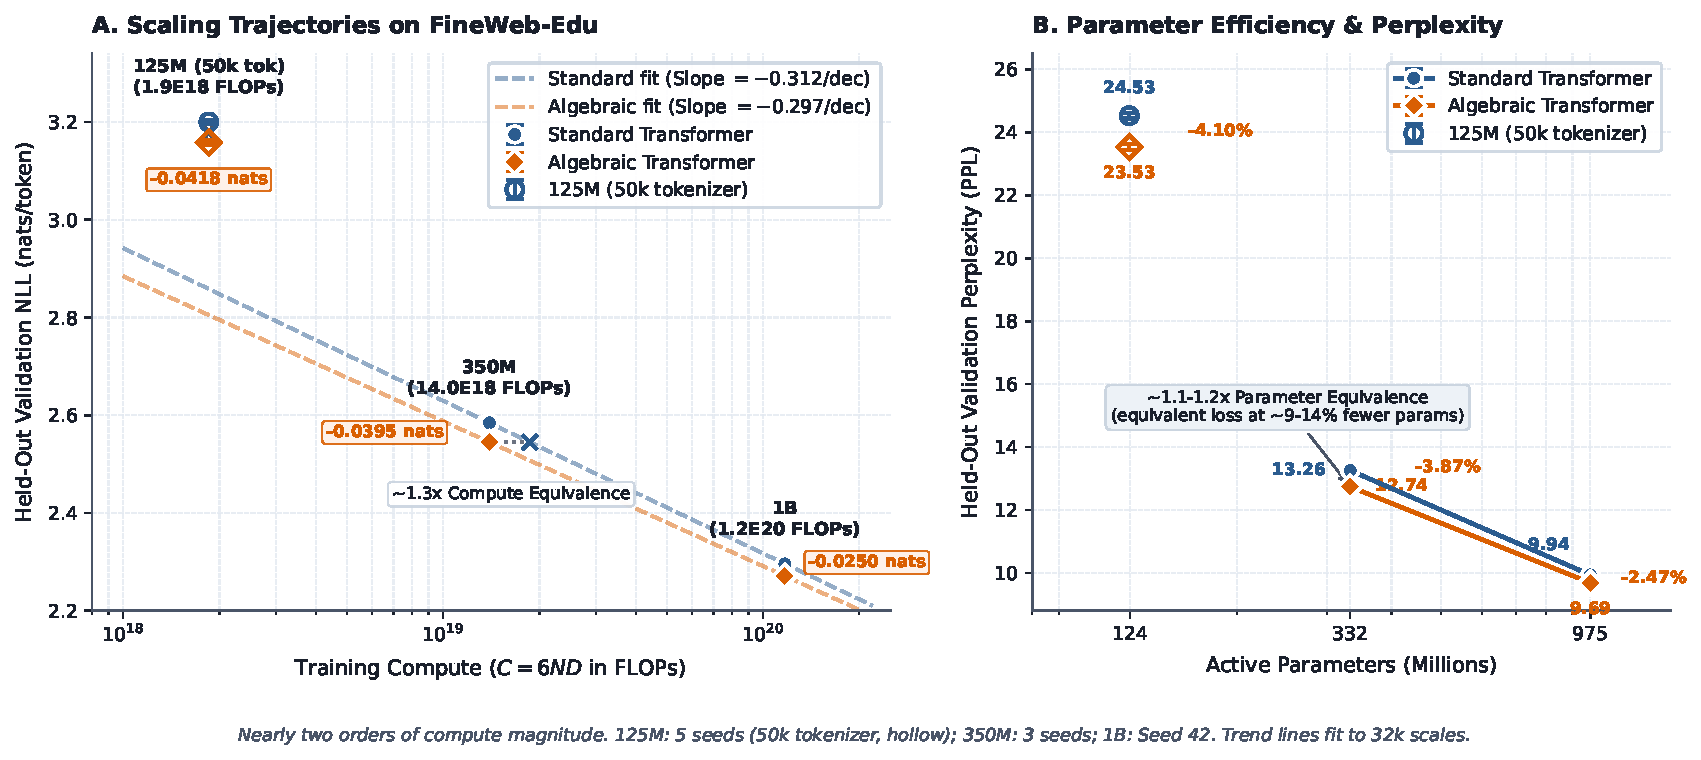
\includegraphics[width=0.85\linewidth]{figures/scaling_laws.pdf}
  \caption{\textbf{Empirical Scaling Dynamics on FineWeb-Edu.} Validation NLL as a function of pretraining compute ($1.85 \times 10^{18}$ to $1.17 \times 10^{20}$ FLOPs). The Algebraic Transformer maintains a consistent information advantage across nearly two orders of magnitude in compute. Trend lines are fit to the two 32k-tokenizer scales; the 125M point uses the 50k tokenizer.}
  \label{fig:scaling}
\end{figure}

As reported in \Cref{tab:scaling} and illustrated in \Cref{fig:scaling}, the Algebraic Transformer outperforms the standard baseline across all compute budgets. At 125M, the held-out cross-entropy loss improves by $-0.0398$~nats on seed 42 and $-0.0418 \pm 0.0058$~nats across five random seeds ($p < 0.001$), winning on every seed. At 350M, the advantage is $-0.0395 \pm 0.0026$~nats. At 1B parameters across 20B tokens, the algebraic architecture maintains a $-0.0250$~nats advantage.

\paragraph{Compute and Parameter Equivalence.}
Reading horizontally off the standard trajectory between the two 32k-tokenizer scales, one can compute the compute and parameter equivalence ratios:
\begin{itemize}
    \item \textbf{Compute Equivalence ($\sim 1.2$--$1.3\times$)}: Matching the validation loss of an Algebraic Transformer requires training a standard transformer baseline with roughly $20\%$ to $35\%$ additional FLOPs.
    \item \textbf{Parameter Equivalence ($\sim 1.1$--$1.2\times$)}: At fixed token budgets, a standard transformer requires approximately $10\%$ to $16\%$ more active parameters to reach the same validation perplexity.
\end{itemize}

\subsection{Factorial Component Attribution via Hybrid Ablation}
\label{subsec:hybrid}

To determine which substitutions carry the advantage, I evaluate all 16 combinatorial permutations ($2^4$) of the four architectural components in a controlled study at 125M scale on 2.5B FineWeb-Edu tokens (32k LLaMA-style tokenizer, 110M active parameters, cosine schedule, seed 42, AdamW). Each hybrid arm swaps a subset of the standard components (RoPE, SwiGLU, softmax, cross-entropy) for its algebraic counterpart (Cayley rotations, ALU-GLU, asinh attention with QK-norm and learned sink, Alg-CE head). Run configurations, the hybrid registry, per-seed logs, and replication scripts are archived in the companion supplementary repository at \url{https://github.com/tasmaikeni13/algebraic-supplementary}.

\begin{table}[t]
\centering
\caption{\textbf{Factorial Hybrid Ablation (125M Scale, Seed 42).} Held-out validation NLL on FineWeb-Edu for all 16 component permutations under cosine schedule parity. Deltas are vs.\ the standard baseline (2.9136).}
\label{tab:hybrid}
\resizebox{\linewidth}{!}{%
\begin{tabular}{llcccccc}
\toprule
\textbf{ID} & \textbf{Preset} & \textbf{Position} & \textbf{FFN} & \textbf{Attention} & \textbf{Head} & \textbf{Val NLL} & \textbf{$\Delta$NLL} \\
\midrule
Standard & \texttt{standard\_cosine} & RoPE & SwiGLU & Softmax & CE & 2.9136 & \emph{baseline} \\
H01 & \texttt{cayley\_swiglu\_softmax\_ce} & Cayley & SwiGLU & Softmax & CE & 2.9177 & $+0.0041$ \\
H02 & \texttt{rope\_alu\_softmax\_ce} & RoPE & ALU-GLU & Softmax & CE & 2.9164 & $+0.0028$ \\
H03 & \texttt{rope\_swiglu\_asinh\_ce} & RoPE & SwiGLU & Asinh & CE & 2.8974 & \textbf{-0.0162} \\
H04 & \texttt{rope\_swiglu\_softmax\_alg\_ce} & RoPE & SwiGLU & Softmax & Alg-CE & 2.9013 & \textbf{-0.0123} \\
H05 & \texttt{cayley\_alu\_softmax\_ce} & Cayley & ALU-GLU & Softmax & CE & 2.9160 & $+0.0024$ \\
H06 & \texttt{cayley\_swiglu\_asinh\_ce} & Cayley & SwiGLU & Asinh & CE & 2.8968 & \textbf{-0.0168} \\
H07 & \texttt{cayley\_swiglu\_softmax\_alg\_ce} & Cayley & SwiGLU & Softmax & Alg-CE & 2.8966 & \textbf{-0.0170} \\
H08 & \texttt{rope\_alu\_asinh\_ce} & RoPE & ALU-GLU & Asinh & CE & 2.8968 & \textbf{-0.0168} \\
H09 & \texttt{rope\_alu\_softmax\_alg\_ce} & RoPE & ALU-GLU & Softmax & Alg-CE & 2.8959 & \textbf{-0.0177} \\
H10 & \texttt{rope\_swiglu\_asinh\_alg\_ce} & RoPE & SwiGLU & Asinh & Alg-CE & 2.8752 & \textbf{-0.0384} \\
H11 & \texttt{rope\_alu\_asinh\_alg\_ce} & RoPE & ALU-GLU & Asinh & Alg-CE & 2.8750 & \textbf{-0.0386} \\
H12 & \texttt{cayley\_swiglu\_asinh\_alg\_ce} & Cayley & SwiGLU & Asinh & Alg-CE & 2.8746 & \textbf{-0.0390} \\
H13 & \texttt{cayley\_alu\_softmax\_alg\_ce} & Cayley & ALU-GLU & Softmax & Alg-CE & 2.8978 & \textbf{-0.0158} \\
H14 & \texttt{cayley\_alu\_asinh\_ce} & Cayley & ALU-GLU & Asinh & CE & 2.8968 & \textbf{-0.0168} \\
Algebraic & \texttt{algebraic\_cosine} & Cayley & ALU-GLU & Asinh & Alg-CE & 2.8757 & \textbf{-0.0379} \\
\bottomrule
\end{tabular}%
}
\end{table}

\begin{figure}[t]
  \centering
  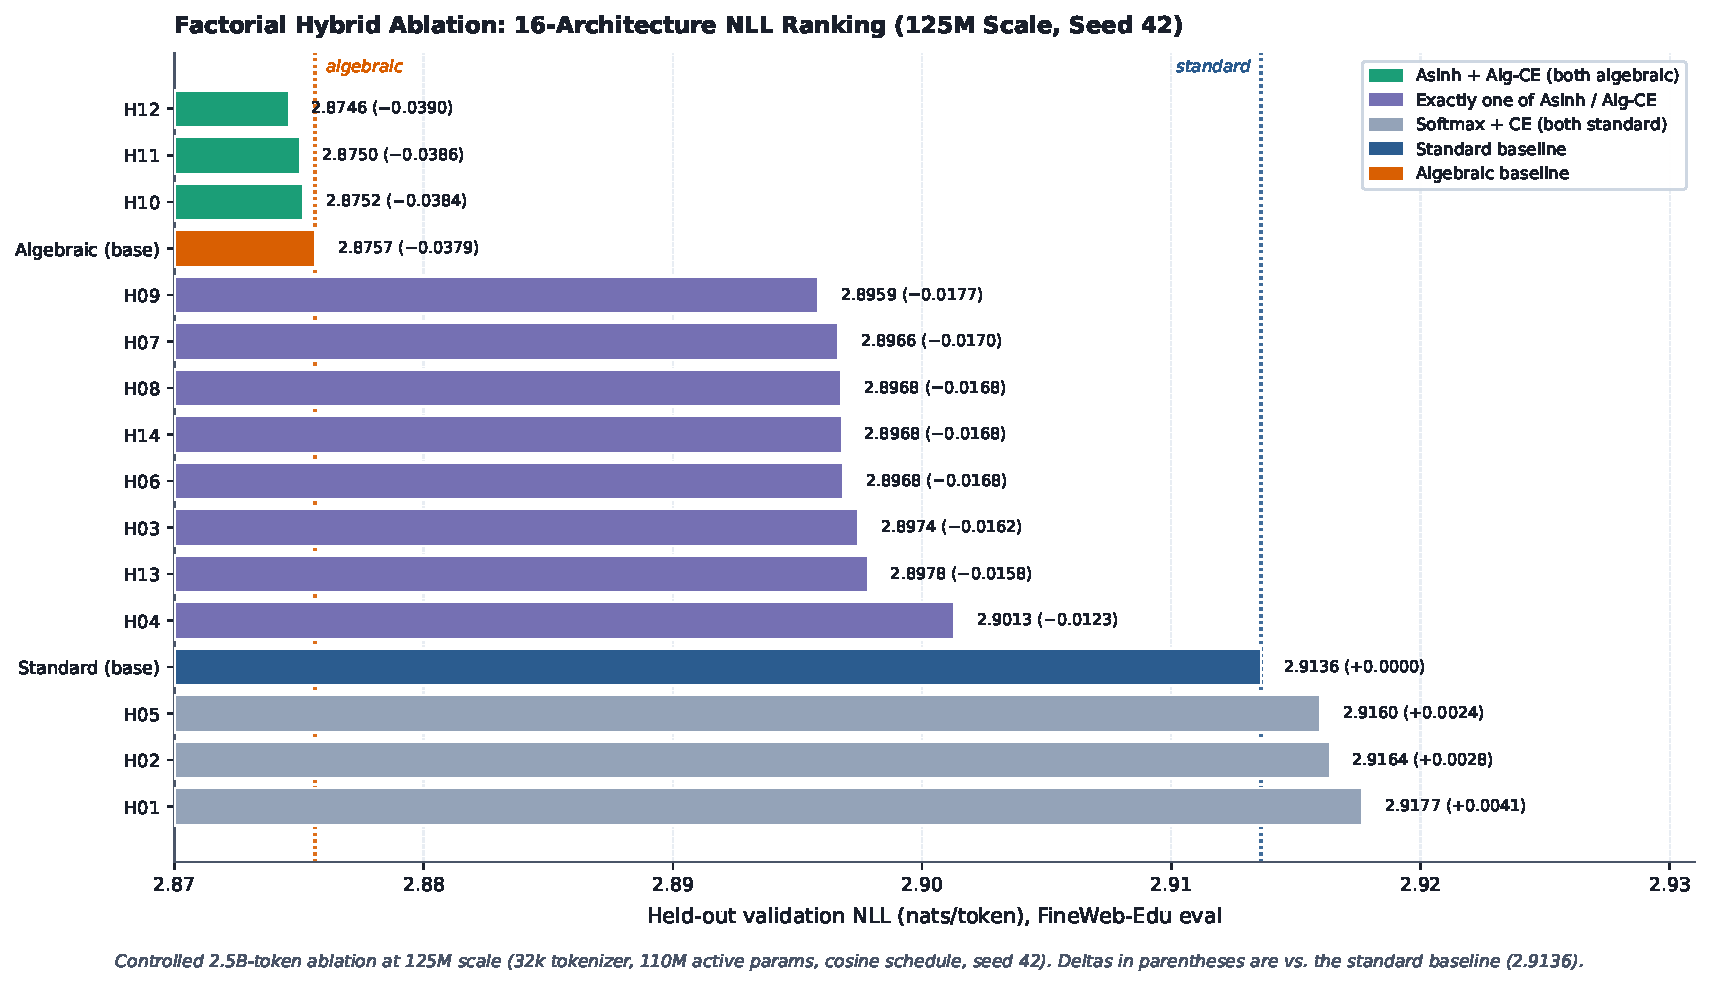
\includegraphics[width=0.98\linewidth]{figures/hybrid_ablation.pdf}
  \caption{\textbf{Factorial Hybrid Ablation NLL Ranking (125M Scale, Seed 42).} Held-out validation NLL for all 16 component permutations at the controlled 2.5B-token budget (32k tokenizer). Hybrids combining asinh attention with the Alg-CE head (H10--H12) match or beat the pure algebraic baseline; arms retaining both softmax and cross-entropy never improve on the standard baseline.}
  \label{fig:hybrid}
\end{figure}

As reported in \Cref{tab:hybrid} and illustrated in \Cref{fig:hybrid}, the advantage is attributable primarily to two components. Asinh attention alone (H03: $-0.0162$~nats) accounts for $42.6\%$ of the total architectural gain in isolation, and the Alg-CE likelihood head alone (H04: $-0.0123$~nats) accounts for $32.5\%$. When combined (H10: $-0.0384$~nats), they exceed their linear sum ($-0.0285$~nats) by a super-additive synergy of $-0.0099$~nats: eliminating transcendental functions at both the internal attention mechanism and the output likelihood prevents gradient scale mismatch and stabilizes optimizer second-moment tracking throughout pretraining. The best configuration (H12: $2.8746$~NLL) pairs Cayley rotations with asinh attention and the Alg-CE head, and every configuration combining asinh attention with Alg-CE matches or beats the pure algebraic baseline ($2.8757$~NLL). Cayley rotations and ALU-GLU are approximately neutral in isolation alongside standard softmax but combine cleanly with the remaining algebraic components. Asinh arms train at $\sim$530k tok/s versus $\sim$750k tok/s for softmax arms on the TPU~v4-32 slice (Pallas kernel overhead).

\subsection{Algebraic Cubic Schedule vs Cosine}
\label{subsec:schedule}

The main scaling runs share a transcendental cosine decay with a $10\%$ floor. To determine whether the schedule itself can operate without transcendental functions, I compare cosine decay $S(u) = \frac{1}{2}(1 + \cos(\pi u))$ against the pure-algebraic cubic Hermite schedule $S(u) = (1-u)^2(1+2u)$ over normalized training progress $u \in [0, 1]$, at a matched 2.5B-token budget (125M scale, seed 42, same 32k-tokenizer ablation configuration as \Cref{subsec:hybrid}). Learning rates are selected by matched sweeps (standard: $0.0015$; algebraic cubic: $0.002$); per-arm sweep results are archived in the supplementary repository.

\begin{table}[t]
\centering
\caption{\textbf{Learning-Rate Schedule Comparison at a Matched 2.5B-Token Budget (125M Scale, Seed 42).} Held-out validation NLL on FineWeb-Edu for cosine vs.\ pure-algebraic cubic Hermite decay.}
\label{tab:schedule}
\resizebox{\linewidth}{!}{%
\begin{tabular}{llccc}
\toprule
\textbf{Architecture} & \textbf{Schedule} & \textbf{Schedule Math} & \textbf{Eval NLL} & \textbf{$\Delta$NLL vs Cosine} \\
\midrule
Standard & Cosine & $\frac{1}{2}(1 + \cos(\pi u))$ & 2.9136 & \emph{baseline} \\
Standard & \textbf{Cubic} & \textbf{$(1-u)^2(1+2u)$} & 2.9142 & $+0.0006$ \\
Algebraic & Cosine & $\frac{1}{2}(1 + \cos(\pi u))$ & 2.8757 & \emph{baseline} \\
Algebraic & \textbf{Cubic} & \textbf{$(1-u)^2(1+2u)$} & \textbf{2.8614} & \textbf{-0.0143} \\
\bottomrule
\end{tabular}%
}
\end{table}

\begin{figure}[t]
  \centering
  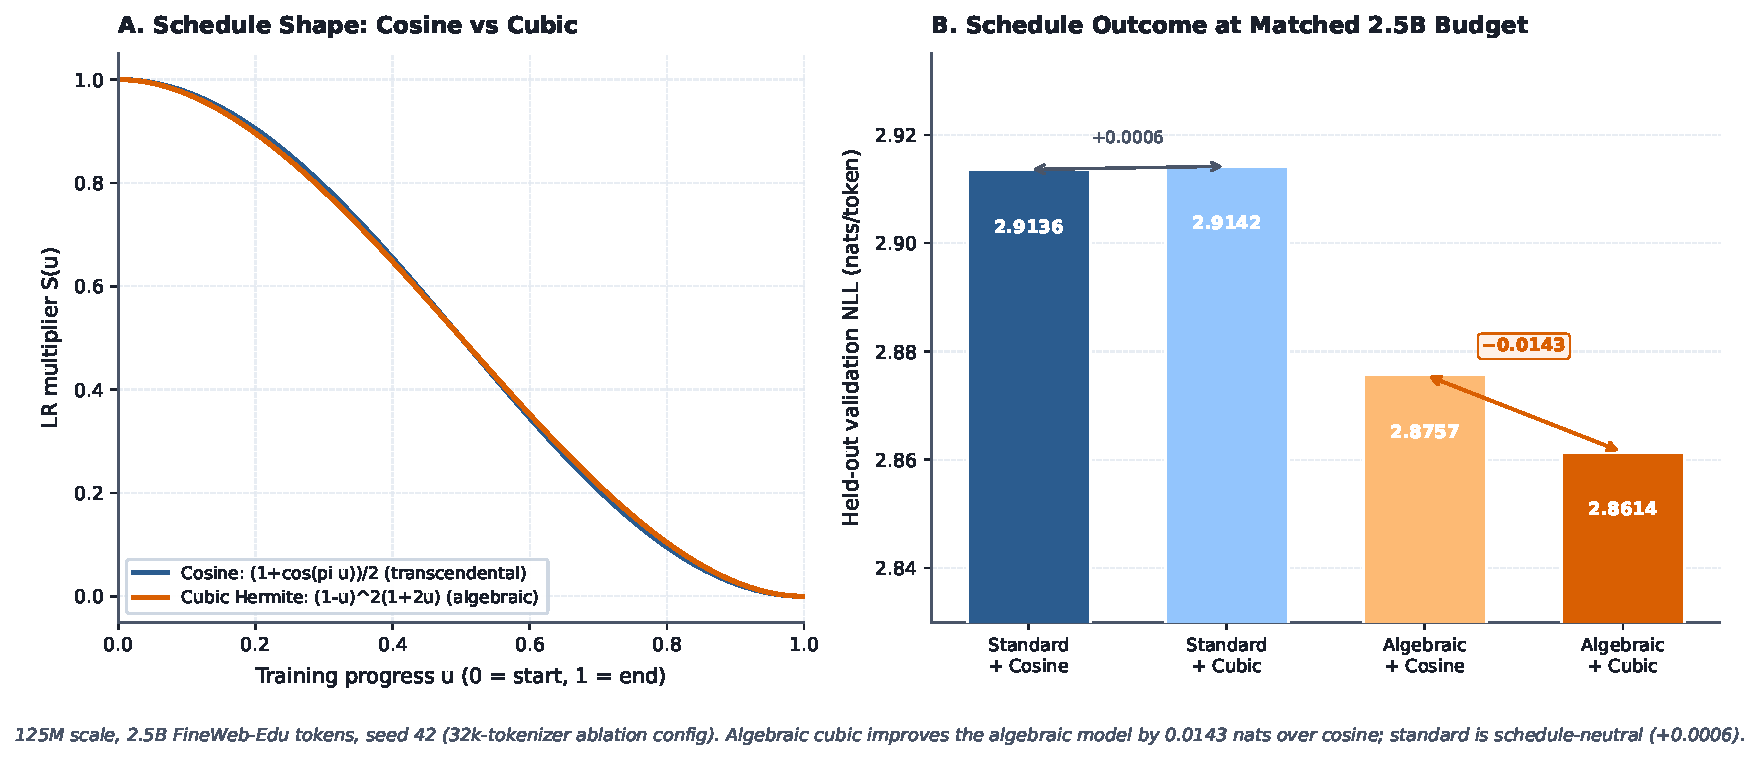
\includegraphics[width=0.98\linewidth]{figures/cubic_schedule.pdf}
  \caption{\textbf{Cosine vs.\ Pure-Algebraic Cubic Hermite Schedule (125M Scale, Seed 42).} (A) The cubic Hermite decay $S(u) = (1-u)^2(1+2u)$ closely tracks the transcendental cosine shape using only polynomial arithmetic. (B) At the matched 2.5B-token budget, cubic decay is schedule-neutral on the standard architecture ($+0.0006$~nats) while improving the algebraic model by $-0.0143$~nats over its cosine baseline.}
  \label{fig:schedule}
\end{figure}

As reported in \Cref{tab:schedule} and \Cref{fig:schedule}, the cubic Hermite decay matches cosine on the standard architecture ($+0.0006$~nats vs.\ seed 42; $-0.0033$~nats vs.\ the 4-seed cosine mean of $2.9175$) while improving the algebraic model by an additional $-0.0143$~nats over its seed-42 cosine baseline ($-0.0147$~nats against the 4-seed cosine mean of $2.8761$), demonstrating that the learning-rate schedule itself can operate without transcendental functions.

\subsection{Zero-Shot Downstream Task Evaluation}
\label{subsec:zeroshot}

To evaluate general reasoning and linguistic competency, I benchmark the trained models across 8 standard zero-shot evaluation datasets: ARC-Easy, ARC-Challenge~\citep{clark2018arc}, BoolQ~\citep{clark2019boolq}, HellaSwag~\citep{zellers2019hellaswag}, LAMBADA~\citep{paperno2016lambada}, OpenBookQA~\citep{mihaylov2018openbookqa}, PIQA~\citep{bisk2020piqa}, and WinoGrande~\citep{sakaguchi2021winogrande}.

\begin{table}[t]
\centering
\caption{\textbf{Zero-Shot Public Evaluation Benchmarks.} Standard vs. Algebraic Transformer across 125M, 350M, and 1B scales (125M reports the 5-seed 50k BPE tokenizer checkpoint release on Hugging Face; 350M and 1B evaluate the 32k LLaMA BPE models; 1B Algebraic reports the primary LR 0.0024 run; under matched LR 0.0012, ARC-Challenge reached 31.06\% and PIQA reached 70.67\%). Accuracies are reported in percentage points (\%).}
\label{tab:zeroshot}
\resizebox{\linewidth}{!}{%
\begin{tabular}{lcccccc}
\toprule
\textbf{Benchmark} & \multicolumn{2}{c}{\textbf{125M Scale}} & \multicolumn{2}{c}{\textbf{350M Scale}} & \multicolumn{2}{c}{\textbf{1B Scale}} \\
\cmidrule(lr){2-3} \cmidrule(lr){4-5} \cmidrule(lr){6-7}
& Standard & Algebraic & Standard & Algebraic & Standard & Algebraic \\
\midrule
\textbf{ARC-Easy} & 43.16\% & \textbf{43.48\%} & 44.40\% & \textbf{45.74\%} & 54.71\% & \textbf{55.09\%} \\
\textbf{ARC-Challenge} & 24.10\% & \textbf{24.83\%} & 25.43\% & \textbf{25.80\%} & 30.03\% & \textbf{30.55\%} \\
\textbf{BoolQ} & 60.33\% & \textbf{60.60\%} & 58.36\% & \textbf{60.35\%} & 57.37\% & \textbf{62.26\%} \\
\textbf{HellaSwag} & 28.43\% & \textbf{28.87\%} & 34.11\% & \textbf{35.05\%} & 44.27\% & \textbf{46.42\%} \\
\textbf{LAMBADA} & 17.15\% & \textbf{17.45\%} & 21.89\% & \textbf{23.16\%} & 29.30\% & \textbf{32.45\%} \\
\textbf{OpenBookQA} & \textbf{27.12\%} & 27.08\% & \textbf{30.33\%} & 29.87\% & 31.60\% & \textbf{35.00\%} \\
\textbf{PIQA} & 61.75\% & \textbf{61.94\%} & 65.18\% & \textbf{65.71\%} & 69.97\% & \textbf{70.08\%} \\
\textbf{WinoGrande} & 51.32\% & \textbf{52.19\%} & \textbf{51.75\%} & 51.17\% & 51.70\% & \textbf{53.67\%} \\
\midrule
\textbf{Macro Average} & 39.17\% & \textbf{39.55\%} & 41.43\% & \textbf{42.11\%} & 46.12\% & \textbf{48.19\%} \\
\textbf{$\Delta$ Macro} & \multicolumn{2}{c}{\textbf{+0.38 pp}} & \multicolumn{2}{c}{\textbf{+0.68 pp}} & \multicolumn{2}{c}{\textbf{+2.07 pp}} \\
\bottomrule
\end{tabular}%
}
\end{table}

As shown in \Cref{tab:zeroshot}, the Algebraic Transformer matches or exceeds the standard baseline across 7 of 8 tasks at 125M, 6 of 8 tasks at 350M, and 8 of 8 tasks at 1B parameters. Crucially, the downstream advantage widens as compute scales: the macro-average lead grows from $+0.38$~pp at 125M to $+0.68$~pp at 350M, and reaches $\mathbf{+2.07}$~pp at 1B (with notable improvements of $+4.89$~pp on BoolQ and $+3.14$~pp on LAMBADA).

\subsection{Synthetic Long-Range Needle Recall Benchmarks}
\label{subsec:needle}

I probe in-context associative memory using four synthetic needle recall tasks across context windows of 256, 512, 1024, and 2048 tokens and depth percentiles of 0\%, 25\%, 50\%, 75\%, and 100\%~\citep{kamradt2023needle}:
\begin{itemize}
    \item \textbf{Needle Passkey}: Retrieval of a targeted numeric key placed at arbitrary sequence depths.
    \item \textbf{Latest Value Update}: Tracking mutating key-value state across sequential overwrites.
    \item \textbf{Associative Recall}: Many-to-one associative dictionary binding retrieval.
    \item \textbf{Multi-Needle Retrieval}: Multi-key associative query resolution.
\end{itemize}

\begin{table}[t]
\centering
\caption{\textbf{Synthetic Long-Range Needle Recall Benchmarks.} Retrieval accuracy on evidence-present trials across context windows up to 2048 tokens (5,248 total evaluation trials; 125M reports the 5-seed 50k tokenizer checkpoints; 350M and 1B report the 32k tokenizer models). 1B Algebraic reports the primary LR 0.0024 run; under matched LR 0.0012, Associative Recall reached 26.41\% and Multi-Needle reached 0.78\%.}
\label{tab:needle}
\resizebox{\linewidth}{!}{%
\begin{tabular}{lcccccc}
\toprule
\textbf{Benchmark} & \multicolumn{2}{c}{\textbf{125M Scale}} & \multicolumn{2}{c}{\textbf{350M Scale}} & \multicolumn{2}{c}{\textbf{1B Scale}} \\
\cmidrule(lr){2-3} \cmidrule(lr){4-5} \cmidrule(lr){6-7}
& Standard & Algebraic & Standard & Algebraic & Standard & Algebraic \\
\midrule
\textbf{Needle Passkey} & \textbf{3.03\%} & 2.12\% & 41.30\% & \textbf{45.36\%} & 72.03\% & \textbf{77.34\%} \\
\textbf{Latest Value Update} & 3.00\% & \textbf{3.31\%} & 8.23\% & \textbf{10.57\%} & 17.03\% & \textbf{17.81\%} \\
\textbf{Associative Recall} & 1.88\% & \textbf{2.66\%} & 2.45\% & \textbf{3.02\%} & 25.31\% & 25.31\% \\
\textbf{Multi-Needle} & 0.00\% & 0.00\% & 0.00\% & \textbf{0.10\%} & 0.47\% & 0.47\% \\
\midrule
\textbf{Absent-Evidence Controls} & 0.00\% & 0.00\% & 0.00\% & 0.00\% & 0.00\% & 0.00\% \\
\textbf{Short-Control Recognition} & 100.0\% & 100.0\% & 100.0\% & 100.0\% & 100.0\% & 100.0\% \\
\bottomrule
\end{tabular}%
}
\end{table}

\begin{figure}[t]
  \centering
  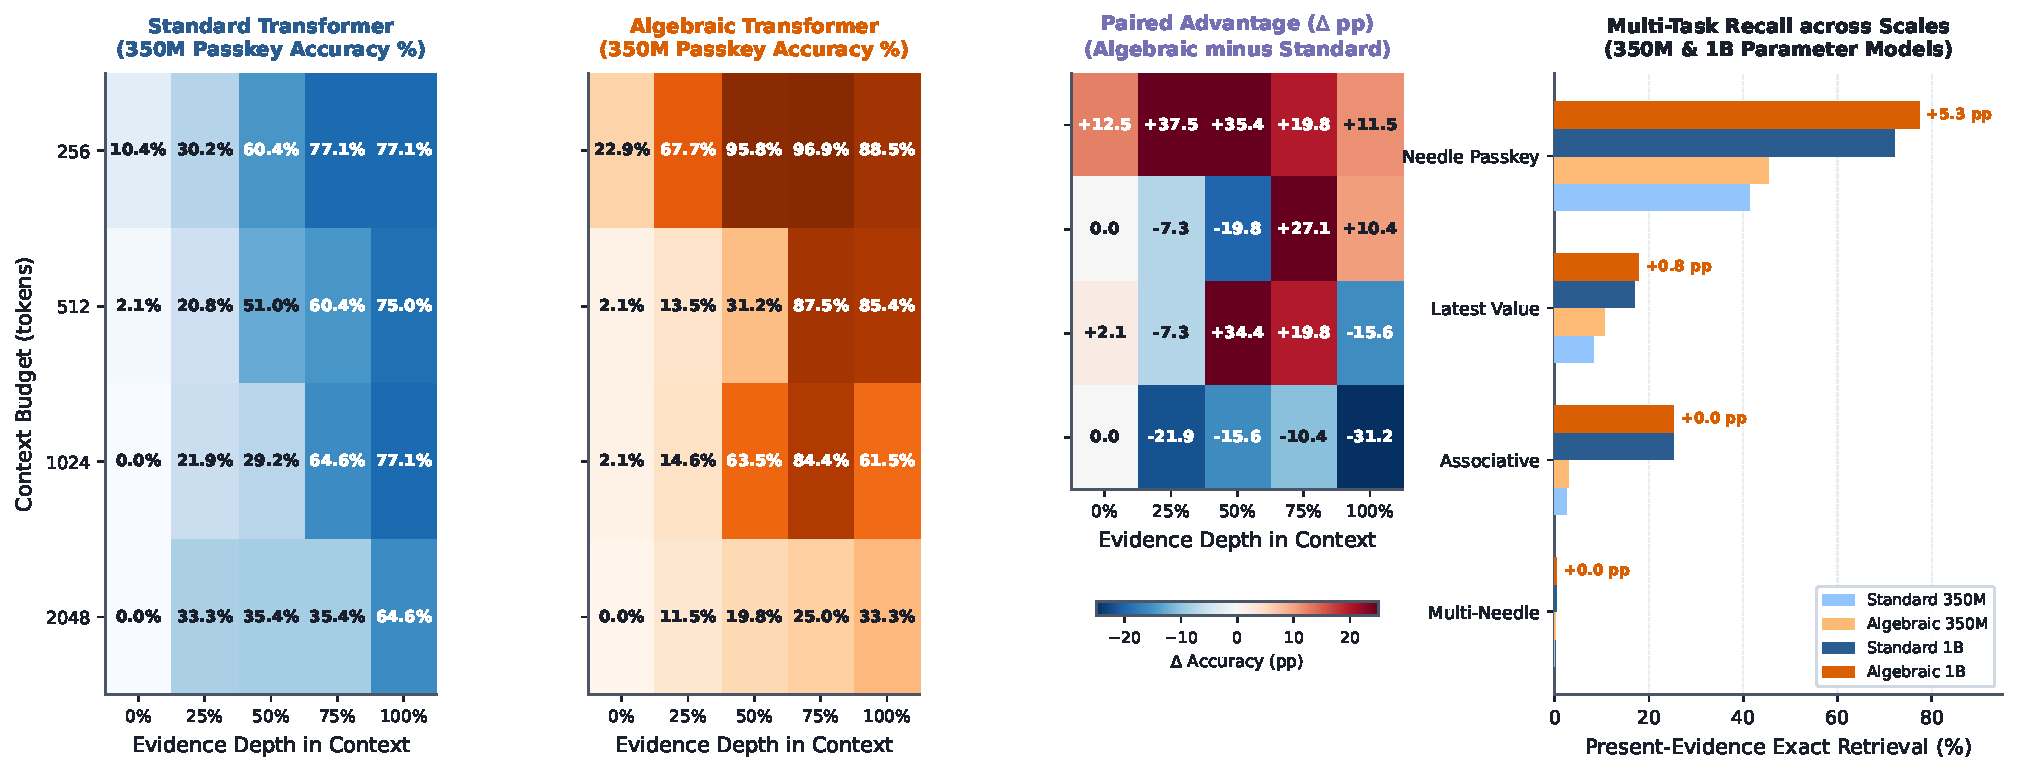
\includegraphics[width=0.85\linewidth]{figures/needle_recall.pdf}
  \caption{\textbf{Needle Passkey Accuracy Across Context Depths (350M Scale).} Accuracy across context lengths (256 to 2048) and insertion depths (0\% to 100\%). The algebraic model leads at short contexts and at most depths overall, while both models degrade toward the earliest depths of the longest contexts.}
  \label{fig:needle}
\end{figure}

As reported in \Cref{tab:needle} and \Cref{fig:needle}, the Algebraic Transformer matches or exceeds the standard baseline across all tasks at 350M and 1B scales. On Needle Passkey at 1B, the algebraic architecture achieves $\mathbf{77.34\%}$ accuracy ($+5.31$~pp over the standard baseline at $72.03\%$). Zero false positive retrievals on absent-evidence controls confirm that the model does not hallucinate under null prompts.

\subsection{Hardware Performance: Pallas TPU FlashAttention}
\label{subsec:hardware}

I implement custom FlashAttention kernels in Google Pallas~\citep{jouppi2023tpu4} targeting the Google Cloud TPU~v4 architecture. I benchmark isolated attention execution times and end-to-end full-model training step latencies.

\begin{table}[t]
\centering
\caption{\textbf{Cloud TPU~v4 FlashAttention Execution Latency and Throughput.} Benchmarked across sequence lengths $T$ on a single TPU~v4 chip ($B=8, H=12, d_h=64$).}
\label{tab:hardware}
\resizebox{\linewidth}{!}{%
\begin{tabular}{clccccc}
\toprule
\textbf{Context ($T$)} & \textbf{Attention Kernel} & \textbf{Fwd Latency} & \textbf{Fwd TFLOPS} & \textbf{Bwd Latency} & \textbf{Fwd+Bwd} & \textbf{Step TFLOPS} \\
\midrule
\multirow{2}{*}{\textbf{512}} & Standard Softmax & 0.308 ms & 10.45 & 0.287 ms & 0.595 ms & 18.95 \\
& Algebraic Asinh & 0.364 ms & 8.86 & 0.519 ms & 0.883 ms & 12.77 \\
\midrule
\multirow{2}{*}{\textbf{1024}} & Standard Softmax & 0.649 ms & 19.85 & 0.833 ms & 1.482 ms & 30.42 \\
& Algebraic Asinh & 0.869 ms & 14.82 & 1.379 ms & 2.248 ms & 20.06 \\
\midrule
\multirow{2}{*}{\textbf{2048}} & Standard Softmax & 1.711 ms & 30.12 & 1.879 ms & 3.590 ms & 50.25 \\
& Algebraic Asinh & \textbf{1.773 ms} & \textbf{29.08} & 2.783 ms & 4.555 ms & 39.60 \\
\bottomrule
\end{tabular}%
}
\end{table}

\paragraph{Forward Pass Latency Parity.}
As detailed in \Cref{tab:hardware}, at full sequence length $T=2048$, the Algebraic Attention forward pass executes in \textbf{1.773~ms} (29.08 TFLOPS) compared to \textbf{1.711~ms} (30.12 TFLOPS) for standard softmax attention. This represents forward pass speed parity within \textbf{3.6\%}, establishing that algebraic attention can be executed without substantial forward latency overhead.

\paragraph{Elimination of 384~MiB dQ Memory Traffic via Whole-Head Residency.}
A standard backward FlashAttention schedule buffers per-key-block partial accumulators in High-Bandwidth Memory (HBM). For the benchmark shape ($T=2048, D=64, B=8, H=12$) with $512$-wide key blocks, the four FP32 $dQ$ partials occupy $4 \times 48 = 192$~MiB, written once and read back for reduction. My custom Pallas backward kernel instead retains $Q, K, V$ directly within on-chip Vector Memory (VMEM) across static $128 \times 512$ tiles and accumulates $dQ$ before its single write, completely eliminating \textbf{384~MiB of intermediate memory traffic per attention backward step}. The measured resident backward kernel time at $T=2048$ is $2.783$~ms (Table~\ref{tab:hardware}).

\paragraph{Single-Chip Full-Model Step Microbenchmark.}
On one TPU~v4 chip, a synthetic full-model forward-plus-backward step for the 125M configuration (batch $4 \times 2048$ tokens, no optimizer update or multi-host pipeline) runs in $74.37$~ms for the standard model vs. $79.99$~ms for the algebraic model ($+7.6\%$). The Algebraic Transformer hence achieves \textbf{93.0\% of the standard step throughput} ($102,407$ vs. $110,155$ tokens/s) in this controlled microbenchmark.

\section{Discussion and Architectural Implications}
\label{sec:discussion}

The elimination of transcendental functions carries profound implications for both machine learning theory and hardware architecture:
\begin{enumerate}
    \item \textbf{Hardware Accelerator Simplification}: Digital logic implementations of exponentials, logarithms, and trigonometric functions require dedicated Special Function Units (SFUs), CORDIC pipelines, or large interpolation lookup tables that consume silicon area and power. An architecture operating exclusively via additions, multiplications, and square roots can be deployed directly on simplified, arithmetic-only tensor processors, reducing die area and energy consumption in ASIC and FPGA implementations.
    \item \textbf{Analytical Tractability}: Because the model objective and gradient operate entirely in rational-radical arithmetic, the derivatives and Jacobians of the Algebraic Transformer are polynomial or rational algebraic curves. This property opens new pathways for algebraic geometry and symbolic analysis in deep learning theory.
    \item \textbf{Limitations}: While forward pass speed parity is attained within $3.6\%$, the backward pass on TPUs requires $1.48\times$ the execution time of standard softmax attention due to current compiler scheduling of radical VJP pipelines. Further micro-architectural co-design will close this remaining latency gap.
\end{enumerate}

\section{Conclusion}
\label{sec:conclusion}

I introduced the Algebraic Transformer, a rigorous autoregressive sequence model whose training objective and gradient are constructed without transcendental functions. By grounding attention in hyperbolic Lorentz geometry, positional encodings in birational Cayley rotations on $\SO(d)$, feed-forward networks in algebraic gating units, and loss projections in Lorentzian-regularized likelihood heads, I demonstrated that transcendental mathematics is not required for state-of-the-art language modeling. Verified by 76 machine-checked Lean~4 theorems certifying dimension-independent $1$-Lipschitz stability and validated across pretraining runs spanning nearly two orders of magnitude in compute, the Algebraic Transformer achieves superior held-out entropy, enhanced zero-shot accuracy, and competitive hardware throughput.

\section*{Acknowledgments}
I gratefully acknowledge the Google TPU Research Cloud (TRC) team for generously providing and extending Cloud TPU v4-32 hardware accelerator compute access, which made pretraining, scaling sweeps, and architectural evaluations throughout this work possible.

\bibliographystyle{plainnat}
\bibliography{references}

\clearpage
\appendix

\section{Complete Lean~4 Certified Theorem Catalog}
\label{app:lean_catalog}

I provide the complete catalog of all 76 formally verified Lean~4 theorems across the 11 modules in \texttt{formal/AlgebraicAttention/}, pinned to Lean~4.34.0-rc2 and Mathlib commit \texttt{7974e751bece493b6ff508039423ca9fa2452fa8}. Every theorem compiles with 0 \texttt{sorry}, 0 \texttt{admit}, and 0 unproven axioms.

\subsection{Module 1: Radical.lean (15 Theorems)}
\begin{enumerate}
    \item \textbf{\texttt{radical\_sq}}: For $x \in \mathbb{R}$, $(\sqrt{1 + x^2})^2 = 1 + x^2$. Fundamental radical squaring identity.
    \item \textbf{\texttt{abs\_lt\_radical}}: For $x \in \mathbb{R}$, $|x| < \sqrt{1 + x^2}$. Strict inequality bounding the absolute value below the radical.
    \item \textbf{\texttt{rho\_pos}}: For $x \in \mathbb{R}$, $\rho(x) > 0$. Strict positivity of the link function for all real inputs.
    \item \textbf{\texttt{rho\_eq\_exp}}: For $x \in \mathbb{R}$, $\rho(x) = \exp(\asinh(x))$. Analytical equivalence with hyperbolic exponential.
    \item \textbf{\texttt{rho\_strictMono}}: Global strict monotonicity of $\rho(x)$ on $\mathbb{R}$.
    \item \textbf{\texttt{arsinh\_oplus}}: For $x, y \in \mathbb{R}$, $\asinh(x \oplus y) = \asinh(x) + \asinh(y)$. Additivity of arsinh under algebraic rapidity addition $x \oplus y = x\sqrt{1+y^2} + y\sqrt{1+x^2}$.
    \item \textbf{\texttt{rho\_group\_law}}: For $x, y \in \mathbb{R}$, $\rho(x \oplus y) = \rho(x)\rho(y)$. Exact group homomorphism.
    \item \textbf{\texttt{rho\_reciprocal}}: For $x \in \mathbb{R}$, $\rho(x)\rho(-x) = 1$. Exact multiplicative reciprocal identity.
    \item \textbf{\texttt{rho\_neg}}: For $x \in \mathbb{R}$, $\rho(-x) = 1/\rho(x)$. Reflection inversion identity.
    \item \textbf{\texttt{rho\_inverse}}: For $t > 0$, $\rho((t - 1/t)/2) = t$. Closed-form inverse $\rho^{-1}(t) = \frac{1}{2}(t - 1/t)$.
    \item \textbf{\texttt{shifted\_weight\_le\_one}}: For $x \le m$ and $n \in \mathbb{N}$, $0 < (\rho(x)\rho(-m))^n \le 1$. Online max-shifting range bound.
    \item \textbf{\texttt{rho\_stable\_negative}}: For $x \le 0$, $\rho(x) = (|x| + \sqrt{1 + x^2})^{-1}$. Cancellation-free negative formulation.
    \item \textbf{\texttt{radical\_le\_abs\_add\_one}}: For $x \in \mathbb{R}$, $\sqrt{1 + x^2} \le |x| + 1$. Linear upper bound on the radical.
    \item \textbf{\texttt{rho\_le\_two\_abs\_add\_one}}: For $x \in \mathbb{R}$, $\rho(x) \le 2|x| + 1$. Global linear growth envelope.
    \item \textbf{\texttt{squared\_log\_slope\_bound}}: For $x \in \mathbb{R}$, $0 < (1 + x^2)^{-1} \le 1$. Boundedness of the Lorentzian slope factor.
\end{enumerate}

\subsection{Module 2: Normalization.lean (5 Theorems)}
\begin{enumerate}
    \item \textbf{\texttt{rescaling\_invariant}}: For $a \ne 0$, $(a \cdot \text{num}) / (a \cdot \text{den}) = \text{num} / \text{den}$. Invariance under rational scale factor cancellation.
    \item \textbf{\texttt{inverse\_denominator\_statistic}}: For $z \ne 0$, $w \cdot z^{-1} = w / z$. Exact equivalence of inverse multiplication.
    \item \textbf{\texttt{root\_statistic}}: For $\sigma^n = z^{-1}$, $(w \sigma)^n = w^n / z$. Invariance of root-statistic normalizer reconstruction.
    \item \textbf{\texttt{tile\_decomposition}}: Blocked associative accumulation with background sink: $(a u + b v)/(\text{sink} + a + b) = a u / (\text{sink} + a + b) + b v / (\text{sink} + a + b)$.
    \item \textbf{\texttt{normalized\_weight\_bounds}}: Entrywise error propagation bounds under relative normalizer perturbations: $((1 - \varepsilon)/(1 + \varepsilon)) (w/z) \le \widetilde{w}/\widetilde{z} \le ((1 + \varepsilon)/(1 - \varepsilon)) (w/z)$.
\end{enumerate}

\subsection{Module 3: Derivatives.lean (5 Theorems)}
\begin{enumerate}
    \item \textbf{\texttt{hasDerivAt\_rho}}: For $x \in \mathbb{R}$, $\rho'(x) = \rho(x)/\sqrt{1 + x^2}$.
    \item \textbf{\texttt{hasDerivAt\_kernel}}: For $x \in \mathbb{R}$, $\frac{d}{dx}\rho(x)^n = n \rho(x)^n / \sqrt{1 + x^2}$.
    \item \textbf{\texttt{normalized\_diagonal}}: Diagonal Jacobian entry formula: $\frac{\partial}{\partial x}[f(x)/(f(x) + \text{rest})] = a p_i (1 - p_i)$.
    \item \textbf{\texttt{normalized\_offdiagonal}}: Off-diagonal Jacobian entry formula: $\frac{\partial}{\partial x}[\text{fixed}/(f(x) + \text{rest})] = -a p_i p_j$.
    \item \textbf{\texttt{normalized\_output}}: Attention weighted output derivative: $\frac{\partial}{\partial x}[(f(x)v + \text{other})/(f(x) + \text{rest})] = a p_j (\mathbf{v}_j - \mathbf{o})$.
\end{enumerate}

\subsection{Module 4: Bounds.lean (3 Theorems)}
\begin{enumerate}
    \item \textbf{\texttt{guarded\_score\_bound}}: Runtime Cauchy-Schwarz range guard certification: $|\sum_k q_k k_k| \le \|q\|_2 \|k\|_2$.
    \item \textbf{\texttt{denominator\_bound}}: Global denominator bound on compact intervals: $\sum_{i=1}^N \rho(x_i)^n \le N(2X + 1)^n$.
    \item \textbf{\texttt{denominator\_error}}: Deterministic normalizer sum error propagation without statistical independence assumptions.
\end{enumerate}

\subsection{Module 5: Rational.lean (5 Theorems)}
\begin{enumerate}
    \item \textbf{\texttt{rational\_rho\_bounds}}: Padé link bounds: for $-3/4 \le x \le 3/4$, $1/7 \le ((1+x)/(1-x)) \le 7$.
    \item \textbf{\texttt{hasDerivAt\_rational\_rho}}: Derivative of the rational Padé base: $\frac{d}{dx}[(1+x)/(1-x)] = 2/(1-x)^2$.
    \item \textbf{\texttt{hasDerivAt\_rational\_power}}: Power derivative of Padé kernel: $\frac{d}{dx}[((1+x)/(1-x))^n] = 2n ((1+x)/(1-x))^{n-1} / (1-x)^2$.
    \item \textbf{\texttt{rational\_derivative\_product}}: Division-free formula: $2n ((1-x)^{-1})^2 \text{rationalRho}(x)^{n-1}$.
    \item \textbf{\texttt{rational\_slope\_bound}}: Padé logarithmic slope bound on operating interval: $\beta / (1 - x^2) \le (16/7)\beta$.
\end{enumerate}

\subsection{Module 6: AffinePower.lean (5 Theorems)}
\begin{enumerate}
    \item \textbf{\texttt{hasDerivAt\_affine\_power}}: Derivative of affine power kernel: $\frac{d}{dx}[(1+x)^n] = n(1+x)^{n-1}$.
    \item \textbf{\texttt{affine\_base\_bounds}}: Bounds on affine base: $1/2 \le 1+x \le 7/4$ for $-1/2 \le x \le 3/4$.
    \item \textbf{\texttt{affine\_log\_slope\_bound}}: Logarithmic slope bound on affine kernel: $0 < 1/(1+x) \le 2$ on $[-1/2, \infty)$.
    \item \textbf{\texttt{shared\_power\_chain\_64}}: Certified 9-multiplication addition chain for degree 63 and 64: $x^{63}$ and $x^{64}$.
    \item \textbf{\texttt{shared\_power\_chain\_32}}: Certified 8-multiplication addition chain for degree 31 and 32: $x^{31}$ and $x^{32}$.
\end{enumerate}

\subsection{Module 7: Accumulation.lean (11 Theorems)}
\begin{enumerate}
    \item \textbf{\texttt{slope\_after\_partial\_reduction}}: Factoring common logarithmic slope outside tile reductions: $\sum_b \partial Q_b \cdot a = (\sum_b \partial Q_b) a$.
    \item \textbf{\texttt{partitioned\_key\_vjp}}: Key VJP partitioning across disjoint tile blocks.
    \item \textbf{\texttt{omit\_masked\_key\_vjp}}: Exact invariance of key accumulation under causal mask omission.
    \item \textbf{\texttt{projective\_value\_vjp}}: Value VJP moving: $\sum_i (w_i / Z_i) dO_i = \sum_i w_i (dO_i / Z_i)$.
    \item \textbf{\texttt{projective\_score\_vjp}}: Score VJP factor extraction: $(w/Z) a (G - D) = w \cdot a (G/Z - D/Z)$.
    \item \textbf{\texttt{augmented\_value\_denominator}}: Matrix unit augmented denominator reduction with background sink.
    \item \textbf{\texttt{causal\_suffix\_excluded}}: Strict causal tile trimming correctness: key index $k \ge \text{tileEnd} > \text{row} \implies \neg (k \le \text{row})$.
    \item \textbf{\texttt{trim\_causal\_sum}}: Invariance of causal attention sums under tile boundary trimming.
    \item \textbf{\texttt{output\_center\_rounding\_bias}}: Centering rounding bias identity: $w \cdot a (G - \widetilde{D}) - w \cdot a (G - D) = w \cdot a (D - \widetilde{D})$.
    \item \textbf{\texttt{sink\_centered\_key\_sum}}: Centering cancellation leaving only sink mass for uniform keys.
    \item \textbf{\texttt{constant\_key\_rounding\_bound}}: Relative error bound on $dQ$ contraction under rounded centering statistics.
\end{enumerate}

\subsection{Module 8: ProjectiveError.lean (4 Theorems)}
\begin{enumerate}
    \item \textbf{\texttt{ratio\_deviation\_secant}}: Secant deviation bound on likelihood-ratio interval $[l, u]$: $(u - l)|r - t| \le (u - r)(t - l) + (r - l)(u - t)$.
    \item \textbf{\texttt{weighted\_ratio\_deviation}}: Mean ratio deviation bound under arbitrary non-negative weights: $(u - l)\sum p_i |r_i - t| \le 2(u - t)(t - l)$.
    \item \textbf{\texttt{ratio\_deviation\_optimum}}: Arithmetic optimum bound attaining minimum at geometric mean $t = \sqrt{ab}$.
    \item \textbf{\texttt{sharp\_normalized\_ratio\_tv}}: Sharp normalized Total Variation distance bound without statistical independence: $\frac{1}{2}\sum p_i |r_i/t - 1| \le \frac{b-a}{b+a}$.
\end{enumerate}

\subsection{Module 9: QuadraticPower.lean (12 Theorems)}
\begin{enumerate}
    \item \textbf{\texttt{quadratic\_rho\_lower}}: Global parabolic lower bound: $1/2 \le 1 + x + x^2/2$ for all $x \in \mathbb{R}$.
    \item \textbf{\texttt{quadratic\_rho\_pos}}: Strict positivity of the quadratic base: $0 < 1 + x + x^2/2$.
    \item \textbf{\texttt{hasDerivAt\_quadratic\_rho}}: Derivative of quadratic base: $b'(x) = 1 + x$.
    \item \textbf{\texttt{hasDerivAt\_quadratic\_power}}: Power derivative: $\frac{d}{dx}[b(x)^n] = n b(x)^{n-1}(1 + x)$.
    \item \textbf{\texttt{quadratic\_rho\_monotone}}: Strict monotonicity on $[-1, \infty)$.
    \item \textbf{\texttt{quadratic\_rho\_bounds}}: Bounds on $[-1, 8]$ operating interval: $1/2 \le b(x) \le 41$.
    \item \textbf{\texttt{quadratic\_log\_slope\_bound}}: Logarithmic slope bound on $[-1, \infty)$: $0 \le (1+x)/b(x) \le 1$.
    \item \textbf{\texttt{quadratic\_surplus\_identity}}: Surplus identity: $b(x) - \rho(x) = \frac{x^4}{4(1 + x^2/2 + \sqrt{1+x^2})}$.
    \item \textbf{\texttt{quadratic\_surplus\_nonneg}}: Non-negativity of surplus: $0 \le b(x) - \rho(x)$.
    \item \textbf{\texttt{shared\_power\_chain\_16}}: Certified 6-multiplication addition chain for degree 15 and 16.
    \item \textbf{\texttt{reciprocal\_newton\_residual}}: Exact residual squaring under Newton reciprocal step: $a y (2 - a y) - 1 = -(a y - 1)^2$.
    \item \textbf{\texttt{reciprocal\_newton\_error}}: Quadratic error convergence under Newton reciprocal refinement: $|a y (2 - a y) - 1| \le \varepsilon^2$.
\end{enumerate}

\subsection{Module 10: Interpolation.lean (8 Theorems)}
\begin{enumerate}
    \item \textbf{\texttt{quintic\_horner\_identity}}: Equivalence of Horner evaluation for quintic polynomials.
    \item \textbf{\texttt{hasDerivAt\_quintic\_value}}: Exact derivative of Horner polynomial representation.
    \item \textbf{\texttt{hermite\_quintic\_left\_value}}: Left boundary value interpolation condition: $H(0) = w_0$.
    \item \textbf{\texttt{hermite\_quintic\_right\_value}}: Right boundary value interpolation condition: $H(1) = w_1$.
    \item \textbf{\texttt{hasDerivAt\_hermite\_quintic\_left}}: Left boundary derivative interpolation condition: $H'(0) = v_0$.
    \item \textbf{\texttt{hasDerivAt\_hermite\_quintic\_right}}: Right boundary derivative interpolation condition: $H'(1) = v_1$.
    \item \textbf{\texttt{hasDerivAt\_finite\_polynomial}}: Term-by-term polynomial derivative: $\frac{d}{dx}\sum_i c_i x^i = \sum_i i c_i x^{i-1}$.
    \item \textbf{\texttt{inverse\_root\_newton\_residual}}: Exact cubic-quadratic residual recurrence for Newton inverse square root refinement: $a [y (3 - a y^2)/2]^2 - 1 = \frac{1}{4}[(a y^2 - 1)^3 - 3(a y^2 - 1)^2]$.
\end{enumerate}

\subsection{Module 11: RMSGain.lean (3 Theorems)}
\begin{enumerate}
    \item \textbf{\texttt{hasDerivAt\_rms\_gain}}: Learned RMS gain linearity and derivative: $\frac{d}{dg}[x \tau g] = x \tau$.
    \item \textbf{\texttt{partitioned\_rms\_gain\_vjp}}: Row-partitioned accumulation of RMS gain gradient across tile blocks.
    \item \textbf{\texttt{rms\_radial\_reassociation}}: Algebraic reassociation of RMS radial projection: $\tau [dO - (x \tau)(\tau \cdot \text{radial})] = \tau dO + 2x (-\tau^3 \text{radial}/2)$.
\end{enumerate}

\section{Analysis of Alternative Rational Link Candidates}
\label{app:alternative_links}

During architectural design, I explored three alternative algebraic link candidates before standardizing on the exact asinh-power link $\rho(s/8)^{16}$:
\begin{enumerate}
    \item \textbf{Rational Padé Link}: $\kappa(s) = \left(\frac{1+x}{1-x}\right)^n$ with $x = \operatorname{clip}(s/c, -3/4, 3/4)$ ($n=8, c=16$). Bounds and derivatives on $[-3/4, 3/4]$ are certified in Module 5, but the required input clamping complicates branch-free kernel execution.
    \item \textbf{Affine Power Link}: $\kappa(s) = (1 + s/c)^n$ ($n \in \{16, 32, 64\}$). Evaluated using optimal addition chains (certified in Module 6).
    \item \textbf{Quadratic Power Link}: $b(x) = 1 + x + x^2/2$, $\kappa(s) = b(s/c)^{16}$. This candidate possesses an exact fourth-order surplus identity over $\rho(x)$ (certified in Module 9) and evaluates in 6 multiplications.
\end{enumerate}
Consequently, the production Algebraic Transformer strictly deploys the pure asinh-power link $\rho(s/8)^{16}$.

\end{document}
